\chapter{Homotopy type theory}
\label{cha:basics}

\section{Types are higher groupoids}
\label{sec:equality}

Recall that for any type $A$, and any $x,y:A$, we have a identity type $\id[A]{x}{y}$, also written $\idtype[A]{x}{y}$ or just $x=y$.
We can think of inhabitants of $x=y$ as either
\begin{enumerate}
\item evidence that $x$ and $y$ are equal,
\item identifications of $x$ with $y$,
\item paths from $x$ to $y$, or
\item isomorphisms/equivalences from $x$ to $y$.
\end{enumerate}
The first is more traditional in type theory; but in homotopy type theory we often take the latter perspectives as well.
It turns out that the defining rules of identity types, as described in the previous chapter, give them structure which corresponds precisely to that of the continuous paths and (higher) homotopies between them in a space, or a (weak) higher-dimensional groupoid.

This interpretation depends on the ability to \emph{iterate} the identity types.
Recall that type theory (unlike, say, first-order logic) does not distinguish between individuals (e.g.\ $x:A$), which may be the subjects of propositions, and proofs of propositions (e.g.\ evidence for $\id[A]{x}{y}$).
Thus, the identity type can be iterated: we can form the type $\id[{\id[A]{x}{y}}]{p}{q}$ of identifications between identifications $p,q$, and the type $\id[{\id[{\id[A]{x}{y}}]{p}{q}}]{r}{s}$, and so on.
(Obviously, the notation ``$\id[A]{x}{y}$'' has its limitations here.
The style $\idtype[A]{x}{y}$ is only slightly better in iterations: $\idtype[{\idtype[{\idtype[A]{x}{y}}]{p}{q}}]{r}{s}$.)

If the  type $A$ is ``set-like'', such as \nat, these iterated identity types will be uninteresting (see \autoref{sec:basics-sets}).
However, under the interpretation of $p,q : \id[A]{x}{y}$ as paths from $x$ to $y$, an element $r : \id[{\id[A]{x}{y}}]{p}{q}$ can be
thought of as a \emph{path between paths}, or a \emph{homotopy}, and visualized as a 2-dimensional path that fills in the space between $p$ and $q$.
Similarly, $\id[{\id[{\id[A]{x}{y}}]{p}{q}}]{r}{s}$ is the type of 3-dimensional paths between two 2-dimensional paths, and so on.
This ``tower of identity types'' is what we claim has the structure of a higher groupoid.

One of the amazing things about homotopy type theory is that all the higher groupoid structure arises automatically from the induction principle for identity types, as stated in \autoref{sec:identity-types}.
Recall that this says that
\begin{itemize}
\item for every $x,y:A$ and every $p:\id[A]xy$ we have a type $D(x,y,p)$, and
\item for every $a:A$ we have an element $d(a):D(a,a,\refl a)$, 
\end{itemize}
then
\begin{itemize}
\item there exists an element $J_{D,d}(x,y,p):D(x,y,p)$ for \emph{every} two elements $x,y:A$ and $p:\id[A]xy$, such that $J_{D,d}(a,a,\refl a) \jdeq d(a)$.
\end{itemize}
In other words, given dependent functions
\begin{align*}
D & :\prd{x,y:A}{p:\id{x}{y}} \type\\
d & :\prd{a:A} D(a,a,\refl{a})
\end{align*}
there is a dependent function
\[J_{D,d}:\prd{x,y:A}{p:\id{x}{y}} D(x,y,p)\]
such that 
\begin{equation}\label{eq:Jconv}
J_{D,d}(a,a,\refl{a})\jdeq d(a)
\end{equation}
for every $a:A$.
The notation $J$ is traditional for this function, but we will not use it very much.
Usually, every time we apply this induction rule we will either not care about the specific function being defined, or we will immediately give it a different name.

Informally, the induction principle for identity types says that if we want to construct an object (or prove a statement) which depends on an inhabitant $p:\id[A]xy$ of an identity type, then it suffices to perform the construction (or the proof) in the special case when $x$ and $y$ are the same (judgmentally) and $p$ is the reflexivity element $\refl{x}:x=x$ (judgmentally).
When writing informally, we may express this with a phrase such as ``by induction, it suffices to assume\dots''.
This reduction to the ``reflexivity case'' is analogous to the reduction to the ``base case'' and ``inductive step'' in an ordinary proof by induction on the natural numbers, and also to the ``left case'' and ``right case'' in a proof by case analysis on a disjoint union or disjunction.

The ``conversion rule''~\eqref{eq:Jconv} is less familiar in the context of proof by induction on natural numbers, but there is an analogous notion in the related concept of definition by recursion.
If a sequence $(a_n)_{n\in \mathbb{N}}$ is defined by giving $a_0$ and specifying $a_{n+1}$ in terms of $a_n$, then in fact the $0^{\mathrm{th}}$ term of the resulting sequence \emph{is} the given one, and the given recurrence relation relating $a_{n+1}$ to $a_n$ holds for the resulting sequence.
(This may seem so obvious as to not be worth saying, but if we view a definition by recursion as an algorithm for calculating values of a sequence, then it is precisely the process of executing that algorithm.)
The rule~\eqref{eq:Jconv} is analogous: it says that if we define an object $f(p)$ for all $p:x=y$ by specifying what the value should be when $p$ is $\refl{x}:x=x$, then the value we specified is in fact the value of $f(\refl{x})$.

We now derive from this induction principle the beginnings of the structure of a higher groupoid.
We begin with symmetry of equality, which, in topological language, means that ``paths can be reversed''.

\begin{lem}\label{lem:opp}
  For every type $A$ and every $x,y:A$ there is a function
  \begin{equation*}
    (x= y)\to(y= x)
  \end{equation*}
  denoted $p\mapsto \opp{p}$, such that $\opp{\refl{x}}\jdeq\refl{x}$ for each $x:A$.
\end{lem}
\begin{proof}[First proof]
  Let $D:\prd{x,y:A}{p:x= y} \type$ be the type family defined by $D(x,y,p)\defeq (y= x)$.
  In other words, $D$ is a function assigning to any $x,y:A$ and $p:x=y$ a type, namely the type $y=x$.
  Then we have an element
  \begin{equation*}
    d\defeq \lam{x} \refl{x}:\prd{x:A} D(x,x,\refl{x}).
  \end{equation*}
  Thus, the eliminator $J$ for identity types gives us an element $J_{D,d}(x,y,p): (y= x)$ for each $p:(x= y)$.
  We can now define the desired function $\opp{(-)}$ to be $\lam{p} J_{D,d}(x,y,p)$, i.e.\ we set $\opp{p} \defeq J_{D,d}(x,y,p)$.
  The conversion rule~\eqref{eq:Jconv} gives $\opp{\refl{x}}\jdeq \refl{x}$, as required.
\end{proof}

We have written out this proof in a very formal style, which may be helpful while the induction rule on identity types is unfamiliar.
However, eventually we prefer to use more natural language, such as in the following equivalent proof.

\begin{proof}[Second proof]
  We want to construct, for each $x,y:A$ and $p:x=y$, an element $\opp{p}:y=x$.
  By induction, it suffices to do this in the case when $y$ is $x$ and $p$ is $\refl{x}$.
  But in this case, the type $x=y$ of $p$ and the type $y=x$ in which we are trying to construct $\opp{p}$ are both simply $x=x$.
  Thus, in the ``reflexivity case'', we can define $\opp{\refl{x}}$ to be simply $\refl{x}$.
  The general case then follows by the induction principle, and the conversion rule $\opp{\refl{x}}\jdeq\refl{x}$ is precisely the proof in the reflexivity case that we gave.
\end{proof}

We will write out the next few proofs in both styles, to help the reader become accustomed to the latter one.
Next we prove the transitivity of equality, or equivalently we ``concatenate paths''.

\begin{lem}\label{lem:concat}
  For every type $A$ and every $x,y,z:A$ there is a function
  \begin{equation*}
  (x= y) \to   \big((y= z)\to (x=  z)\big)
  \end{equation*}
  written $(p,q)\mapsto p\ct q$, such that $\refl{x}\ct \refl{x}\jdeq \refl{x}$ for any $x:A$.
\end{lem}

\begin{proof}[First proof]
  Let $D:\prd{x,y:A}{p:x=y} \type$ be the type family
  \begin{equation*}
    D(x,y,p)\defeq \prd{z:A}{q:y=z} (x=z).
  \end{equation*}
  Note that $D(x,x,\refl x) \jdeq \prd{z:A}{q:x=z} (x=z)$.
  Thus, in order to apply the induction principle for identity types to this $D$, we need a function of type
  \begin{equation}\label{eq:concatD}
    \prd{x:A} D(x,x,\refl{x})
  \end{equation}
  which is to say, of type
  \[ \prd{x,z:A}{q:x=z} (x=z). \]
  Now let $E:\prd{x,z:A}{q:x=z}\type$ be the type family $E(x,z,q)\defeq (x=z)$.
  Note that $E(x,x,\refl x) \jdeq (x=x)$.
  Thus, we have the function
  \begin{equation*}
    e(x) \defeq \refl{x} : E(x,x,\refl{x}).
  \end{equation*}
  By the induction principle for identity types applied to $E$, we obtain a function
  \begin{equation*}
    d(x,z,q) : \prd{x,z:A}{q:x=z} E(x,z,q).
  \end{equation*}
  But $E(x,z,q)\jdeq (x=z)$, so this is~\eqref{eq:concatD}.
  Thus, we can use this function $d$ and apply the induction principle for identity types to $D$, to obtain our desired function of type
  \begin{equation*}
    \prd{x,y,z:A}{q:y=z}{p:x=y} (x=z).
  \end{equation*}
  The conversion rules for the two induction principles give us $\refl{x}\ct \refl{x}\jdeq \refl{x}$ for any $x:A$.
\end{proof}

\begin{proof}[Second proof]
  We want to construct, for every $x,y,z:A$ and every $p:x=y$ and $q:y=z$, an element of $x=z$.
  By induction on $p$, it suffices to assume that $y$ is $x$ and $p$ is $\refl{x}$.
  In this case, the type $y=z$ of $q$ is $x=z$.
  Now by induction on $q$, it suffices to assume also that $z$ is $x$ and $q$ is $\refl{x}$.
  But in this case, $x=z$ is $x=x$, and we have $\refl{x}:(x=x)$.
\end{proof}

The reader may well feel that we have given an overly convoluted proof of this lemma.
In fact, we could stop after the induction on $p$, since at that point what we want to produce is an equality $x=z$, and we already have such an equality, namely $q$.
Why do we go on to do another induction on $q$?

The answer is that, as described in the introduction, we are doing \emph{proof-relevant} mathematics.
When we prove a lemma, we are defining an inhabitant of some type, and it can matter what \emph{specific} element we defined in the course of the proof, not merely the type that that element inhabits (that is, the \emph{statement} of the lemma).
\autoref{lem:concat} has three obvious proofs: we could do induction over $p$, induction over $q$, or induction over both of them.
If we proved it three different ways, we would have three different elements of the same type.
It's not hard to show that these three elements are equal (see \autoref{ex:basics:concat}), but as they are not \emph{definitionally} equal, there can still be reasons to prefer one over another.

In the case of \autoref{lem:concat}, the difference hinges on the computation rule.
If we proved the lemma using a single induction over $p$, then we would end up with a computation rule of the form $\refl{y} \ct q \jdeq q$.
If we proved it with a single induction over $q$, we would have instead $p\ct\refl{x}\jdeq p$, while proving it with a double induction (as we did) gives only $\refl{x}\ct\refl{x} \jdeq \refl{x}$.

The asymmetrical computation rules can sometimes be convenient when doing formalized mathematics, as they allow the computer to simplify more things automatically.
However, in informal mathematics, and arguably even in the formalized case, it can be confusing to have a concatenation operation which behaves asymmetrically and to have to remember which side is the ``special'' one.
Treating both sides symmetrically makes for more robust proofs; this is why we have given the proof that we did.
(However, this is admittedly a stylistic choice.)

The table below summarizes the ``equality'' and ``homotopical'' points of view on what we have done so far.
\begin{center}
  \begin{tabular}{c|c}
    Equality & Homotopy \\\hline
    reflexivity & constant path\\
    symmetry & inversion of paths\\
    transitivity & concatenation of paths
  \end{tabular}
\end{center}

Because of proof-relevance, we can't stop after proving ``symmetry'' and ``transitivity'' of equality: we need to know that these \emph{operations} on equalities are well-behaved.
(This issue is invisible in set theory, where symmetry and transitivity are mere \emph{properties} of equality, rather than structure on
paths.)
From the homotopy-theoretic point of view, concatenation and inversion are just the ``first level'' of higher groupoid structure --- we also need coherence laws on these operations, and analogous operations at higher dimensions.
For instance, we need to know that concatenation is \emph{associative}, and that inversion provides \emph{inverses} with respect to concatenation.

\begin{lem}\label{thm:omg}%[The $\omega$-groupoid structure of types]
  Suppose $A:\type$, that $x,y,z,w:A$ and that $p:x= y$ and $q:y = z$ and $r:z=w$.
  We have the following:
  \begin{enumerate}
  \item $p= p\ct \refl{y}$ and $p = \refl{x} \ct p$.\label{item:omg1}
  \item $\opp{p}\ct p=  \refl{y}$ and $p\ct \opp{p}= \refl{x}$.
  \item $\opp{(\opp{p})}= p$.
  \item $p\ct (q\ct r)=  (p\ct q)\ct r$.\label{item:omg4}
  \end{enumerate}
\end{lem}

Note, in particular, that~\ref{item:omg1}--\ref{item:omg4} are themselves propositional equalities, living in the identity types \emph{of} identity types, such as $p=_{x=y}q$ for $p,q:x=y$.
Topologically, they are \emph{paths of paths}, i.e.\ homotopies.
It is a familiar fact in topology that when we concatenate a path $p$ with the reversed path $\opp p$, we don't literally obtain a constant path (which corresponds to the equality $\refl{}$ in type theory) --- instead we have a homotopy, or higher path, from $p\ct\opp p$ to the constant path.

\begin{proof}[Proof of~\autoref{thm:omg}]
  All the proofs use the induction principle for equalities.
  \begin{enumerate}
  \item \emph{(First proof)} Let $D:\prd{x,y:A}{p:x=y} \type$ be the type family given by 
    \begin{equation*}
      D(x,y,p)\defeq (p= p\ct \refl{y}).
    \end{equation*}
    Then $D(x,x,\refl{x})$ is $\refl{x}=\refl{x}\ct\refl{x}$.
    Since $\refl{x}\ct\refl{x}\jdeq\refl{x}$, it follows that $D(x,x,\refl{x})\jdeq (\refl{x}=\refl{x})$.
    Thus, there is a function
    \begin{equation*}
      d\defeq\lam{x} \refl{\refl{x}}:\prd{x:A} D(x,x,\refl{x}).
    \end{equation*}
    Now the induction principle for identity types gives an element $J(D,d,p):(p= p\ct\refl{y})$ for each $p:x= y$.
    The other equality is proven similarly.

    \noindent
    \emph{(Second proof)} By induction on $p$, it suffices to assume that $y$ is $x$ and that $p$ is $\refl x$.
    But in this case, we have $\refl{x}\ct\refl{x}\jdeq\refl{x}$.
  \item \emph{(First proof)} Let $D:\prd{x,y:A}{p:x=y} \type$ be the type family given by 
    \begin{equation*}
      D(x,y,p)\defeq (\opp{p}\ct p=  \refl{y}).
    \end{equation*}
    Then $D(x,x,\refl{x})$ is $\opp{\refl{x}}\ct\refl{x}=\refl{x}$.
    Since $\opp{\refl{x}}\jdeq\refl{x}$ and $\refl{x}\ct\refl{x}\jdeq\refl{x}$, we get that $D(x,x,\refl{x})\jdeq (\refl{x}=\refl{x})$.
    Hence we find the function
    \begin{equation*}
      d\defeq\lam{x} \refl{\refl{x}}:\prd{x:A} D(x,x,\refl{x}).
    \end{equation*}
    Now path induction gives an element $J(D,d,p):\opp{p}\ct p=\refl{y}$ for each $p:x= y$ in $A$.
    The other equality is similar.

    \noindent \emph{(Second proof)} By induction, it suffices to assume $p$ is $\refl x$.
    But in this case, we have $\opp{p} \ct p \jdeq \opp{\refl x} \ct \refl x \jdeq \refl x$.
  \item \emph{(First proof)} Let $D:\prd{x,y:A}{p:x=y} \type$ be the type family given by
    \begin{equation*}
      D(x,y,p)\defeq (\opp{\opp{p}}= p).
    \end{equation*}
    Then $D(x,x,\refl{x})$ is the type $(\opp{\opp{\refl x}}=\refl{x})$.
    But since $\opp{\refl{x}}\jdeq \refl{x}$ for each $x:A$, we have $\opp{\opp{\refl{x}}}\jdeq \opp{\refl{x}} \jdeq\refl{x}$, and thus $D(x,x,\refl{x})\jdeq(\refl{x}=\refl{x})$.
    Hence we find the function
    \begin{equation*}
      d\defeq\lam{x} \refl{\refl{x}}:\prd{x:A} D(x,x,\refl{x}).
    \end{equation*}
    Now path induction gives an element $J(D,d,p):\opp{\opp{p}}= p$ for each $p:x= y$.

    \noindent \emph{(Second proof)} By induction, it suffices to assume $p$ is $\refl x$.
    But in this case, we have $\opp{\opp{p}}\jdeq \opp{\opp{\refl x}} \jdeq \refl x$.
  \item \emph{(First proof)} Let $D_1:\prd{x,y:A}{p:x=y} \type$ be the type family given by
    \begin{equation*}
      D_1(x,y,p)\defeq\prd{z,w:A}{q:y= z}{r:z= w} \big(p\ct (q\ct r)=  (p\ct q)\ct r\big).
    \end{equation*}
    Then $D_1(x,x,\refl{x})$ is
    \begin{equation*}
      \prd{z,w:A}{q:x= z}{r:z= w} \big(\refl{x}\ct(q\ct r)= (\refl{x}\ct q)\ct r\big).
    \end{equation*}
    To construct an element of this type, let $D_2:\prd{x,z:A}{q:x=z} \type$ be the type family
    \begin{equation*}
      D_2 (x,z,q) \defeq \prd{w:A}{r:z=w} \big(\refl{x}\ct(q\ct r)= (\refl{x}\ct q)\ct r\big).
    \end{equation*}
    Then $D_2(x,x,\refl{x})$ is
    \begin{equation*}
      \prd{w:A}{r:x=w} \big(\refl{x}\ct(\refl{x}\ct r)= (\refl{x}\ct \refl{x})\ct r\big).
    \end{equation*}
    To construct an element of \emph{this} type, let $D_3:\prd{x,w:A}{r:x=w} \type$ be the type family
    \begin{equation*}
      D_3(x,w,r) \defeq \big(\refl{x}\ct(\refl{x}\ct r)= (\refl{x}\ct \refl{x})\ct r\big).
    \end{equation*}
    Then $D_3(x,x,\refl{x})$ is
    \begin{equation*}
      \big(\refl{x}\ct(\refl{x}\ct \refl{x})= (\refl{x}\ct \refl{x})\ct \refl{x}\big)
    \end{equation*}
    which is definitionally equal to the type $(\refl{x} = \refl{x})$, and is therefore inhabited by $\refl{\refl{x}}$.
    Applying the identity elimination rule three times, therefore, we obtain an element of the overall desired type.

    \noindent \emph{(Second proof)} By induction, it suffices to assume $p$, $q$, and $r$ are all $\refl x$.
    But in this case, we have
    \begin{align*}
      p\ct (q\ct r)
      &\jdeq \refl{x}\ct(\refl{x}\ct \refl{x})\\
      &\jdeq \refl{x}\\
      &\jdeq (\refl{x}\ct \refl x)\ct \refl x\\
      &\jdeq (p\ct q)\ct r.
    \end{align*}
    Thus, we have $\refl{\refl{x}}$ inhabiting this type.\qedhere
  \end{enumerate}
\end{proof}

\begin{rmk}
  There are other ways to define all of these higher paths.
  For instance, in \autoref{thm:omg}\ref{item:omg4} we might do induction only over one or two paths rather than all three.
  Each possibility will produce a \emph{definitionally} different proof, but they will all be equal to each other.
  Such an equality between any two particular proofs can, again, be proven by induction, reducing all the paths in question to reflexivities and then observing that both proofs reduce themselves to reflexivities.
\end{rmk}

We are still not really done with the higher groupoid structure: the paths~\ref{item:omg1}--\ref{item:omg4} must also satisfy their own higher coherence laws, which are themselves higher paths, and so on ``all the way up to infinity" (this is made precise using e.g.\ the the notion of a globular operad).
However, for most purposes it is unnecessary to make the whole infinite-dimensional structure explicit.
One of the nice things about homotopy type theory is that all of this structure can be \emph{proven} starting from only the inductive property of identity types, so we can make explicit as much or as little of it as we need.
In particular, in this book we will not need any of the complicated combinatorics involved in making precise notions such as ``coherent structure at all higher levels''.

One particularly important case of iterated identity types (path types) is when the start and end points are the same.
In set theory, the propositon $a=a$ is entirely uninteresting, but in homotopy theory paths from a point to itself are called \emph{loops} and carry lots of interesting higher structure.
Thus, given a type $A$ with a point $a:A$, we define its \emph{loop space} $\Omega(A,a)$ to be the type $\id[A]{a}{a}$.
We may sometimes write simply $\Omega A$ if the point $a$ is understood from context.

Since any two elements of $\Omega A$ are paths with the same start and end points, they can be concatenated;
thus we have an operation $\Omega A\times \Omega A\to \Omega A$.
More generally, the higher groupoid structure of $A$ gives $\Omega A$ the analogous structure of a ``higher group''.

It can also be useful to consider the loop space \emph{of} the loop space of $A$, which is the space of 2-dimensional loops on the identity loop in $a$.
This is written $\Omega^2(A,a)$ and represented in type theory by the type $\id[{\id[A]{a}{a}}]{\refl{a}}{\refl{a}}$.
And so on.
In general, we make the following definitions:

\begin{defn} \label{def:pointedtype}
  A \textbf{pointed type} $(A,a)$ is a type $A:\type$ together with a point $a:A$.
  We write $\pointed{\type} \defeq \sm{A:\type} A$ for the type of pointed types in the universe $\type$.
\end{defn}

\begin{defn} \label{def:loopspace}
  Given a pointed type $(A,a)$, we define the \textbf{loop space} of $(A,a)$ to be the following pointed type:
  \[\Omega(A,a)=((\id[A]aa),\refl{A}(a)).\]
  For $n:\N$, the \textbf{$n$-fold iterated loop space} of a pointed type $(A,a)$ is defined recursively by:
  \begin{align*}
    \Omega^0(A,a)&=(A,a)\\
    \Omega^{n+1}(A,a)&=\Omega^n(\Omega(A,a)).
  \end{align*}
\end{defn}

We will return to iterated loop spaces in \autoref{cha:hlevels,cha:hits,cha:homotopy}.


\section{Functions are functors}
\label{sec:functors}

Now we wish to establish that functions $f:A\to B$ behave functorially on paths.
In traditional type theory, this is equivalently the statement that functions respect equality.
Topologically, this corresponds to saying that every function is ``continuous'', i.e.\ preserves paths.

\begin{lem}\label{lem:map}
  Suppose that $f:A\to B$ is a function.
  Then for any $x,y:A$ there is an operation
  \begin{equation*}
    \apfunc f : (x=_A y) \to (f(x)=_B f(y)).
  \end{equation*}
  Moreover, for each $x:A$ we have $\apfunc{f}(\refl{x})\jdeq \refl{f(x)}$.
\end{lem}

The notation $\apfunc f$ can be read either as the \underline{ap}plication of $f$ to a path, or as the \underline{a}ction on \underline{p}aths of $f$.

\begin{proof}[First proof]
  Let $D:\prd{x,y:A}{p:x=y}\type$ be the type family defined by
  \[D(x,y,p)\defeq (f(x)= f(y)).\]
  Then we have
  \begin{equation*}
    d\defeq\lam{x} \refl{f(x)}:\prd{x:A} D(x,x,\refl{x}).
  \end{equation*}
  Applying $J$, we obtain $\apfunc f : \prd{x,y:A}{p:x=y}(f(x)=g(x))$.
  The conversion rule implies $\apfunc f({\refl{x}})\jdeq\refl{f(x)}$ for each $x:A$.
\end{proof}

\begin{proof}[Second proof]
  By induction, it suffices to assume $p$ is $\refl{x}$.
  In this case, we may define $\apfunc f(p) \defeq \refl{f(x)}:f(x)\jdeq f(x)$.
\end{proof}

We will often write $\apfunc f (p)$ as simply $\ap f p$.
This is strictly speaking ambiguous, but generally no confusion arises.
It matches the common convention in category theory of using the same symbol for the application of a functor to objects and to morphisms.

We note that $\apfunc{}$ behaves functorially, in all the ways that one might expect.

\begin{lem}\label{lem:ap-functor}
  For functions $f:A\to B$ and $g:B\to C$ and paths $p:\id[A]xy$ and $q:\id[b]yz$, we have:
  \begin{enumerate}
  \item $\apfunc f(p\ct q) = \apfunc f(p) \ct \apfunc f(q)$.\label{item:apfunctor-ct}
  \item $\apfunc f(\opp p) = \opp{\apfunc f (p)}$.\label{item:apfunctor-opp}
  \item $\apfunc g (\apfunc f(p)) = \apfunc{g\circ f} (p)$.\label{item:apfunctor-compose}
  \end{enumerate}
\end{lem}
\begin{proof}
  Left to the reader.
\end{proof}

Now, since \emph{dependently typed} functions are essential in type theory, we will also need a version of \autoref{lem:map} for these.
However, this is not quite so simple to state, because if $f:\prd{x:A} B(x)$ and $p:x=y$, then $f(x):B(x)$ and $f(y):B(y)$ are elements of distinct types, so that \emph{a priori} we cannot even ask whether they are equal.
The missing ingredient is that $p$ itself gives us a way to relate the types $B(x)$ and $B(y)$.

\begin{lem}[Transport]\label{lem:transport}
  Suppose that $P$ is a type family over $A$ and that $p:\id[A]xy$.
  Then there is a function $\transf{p}:P(x)\to P(y)$.
\end{lem}

\begin{proof}[First proof]
  Let $D:\prd{x,y:A}{p:\id{x}{y}} \type$ be the type family defined by
  \[D(x,y,p)\defeq P(x)\to P(y).\]
  Then we have the function
  \begin{equation*}
    d\defeq\lam{x} \idfunc[P(x)]:\prd{x:A} D(x,x,\refl{x}),
  \end{equation*}
  so that the induction principle gives us $J_{D,d}(x,y,p):P(x)\to P(y)$ for $p:x= y$, which we define to be $\transf p$.
\end{proof}

\begin{proof}[Second proof]
  By induction, it suffices to assume $p$ is $\refl x$.
  But in this case, we can take $\transf{(\refl x)}:P(x)\to P(x)$ to be the identity function.
\end{proof}

Sometimes, it is necessary to notate the type family $P$ in which the transport operation happens.
In this case, we may write
\[\transfib P p - : P(x) \to P(y).\]

Recall that a type family $P$ over a type $A$ can be seen as a property of elements of $A$, which holds at $x$ in $A$ if $P(x)$ is inhabited.
Then the transportation lemma says that $P$ respects equality, in the sense that if $x$ is equal to $y$, then $P(x)$ holds if and only if $P(y)$ holds.
In fact, we will see later on that if $x=y$ then actually $P(x)$ and $P(y)$ are \emph{equivalent}.

Topologically, the transportation lemma can be viewed as a ``path lifting'' operation in a fibration.
Given a path $p:x=y$ in the base space $A$ and a point $u:P(x)$ in the fiber over $x$, we may lift the path $p$ to a path in the total space starting at $u$.
The point $\trans p u$ is the other endpoint of this lifted path.
We can also define the path itself in type theory:

\begin{lem}[Path lifting property]\label{thm:path-lifting}
  Let $P:A\to\type$ be a type family over $A$ and assume we have $u:P(x)$ for some $x:A$.
  Then for any $p:x=y$, we have
  \begin{equation*}
    \mathsf{lift}(u,p):(x,u)=(y,\trans{p}{u})
  \end{equation*}
  in $\sm{x:A}P(x)$.
\end{lem}
\begin{proof}
  Left to the reader.
  We will prove a more general theorem in \autoref{sec:compute-sigma}.
\end{proof}

% \begin{proof}[First proof]
% Let $D:\prd{x,y:A}{p:x=y}\type$ be defined by
% \begin{equation*}
% D(x,y,p)\defeq (x,u)=(y,\trans{p}{u}).
% \end{equation*}
% Then $D(x,x,\refl{x})\defeq (x,u)=(x,\trans{\refl{x}}{u})$. By the conversion rule we have $\trans{\refl{x}}{u}\defeq u$, so we see that $D(x,x,\refl{x})\defeq (x,u)=(x,u)$. Therefore we find $d(x)\defeq\refl{(x,u)}:D(x,x,\refl{x})$. Now path induction gives a function of type $\prd{x,y:A}{p:x=y}(x,u)=(y,\trans{p}{u})$.
% \end{proof}
% \begin{proof}[Second proof] 
%   By induction, it suffices to find an element of $(x,u)=(x,\trans{\refl{x}}{u})$.
%   Note that $\trans{\refl{x}}{u}\jdeq u$, so we really need to find an element of $(x,u)=(x,u)$.
%   But here we can use reflexivity.
% \end{proof}

Now we can prove the dependent version of \autoref{lem:map}.
The topological intuition is that given $f:\prd{x:A} P(x)$ and a path $p:\id[A]xy$, we ought to be able to apply $f$ to $p$ and obtain a path in the total space of $P$ which ``lies over'' $p$, as shown below.

\begin{center}
  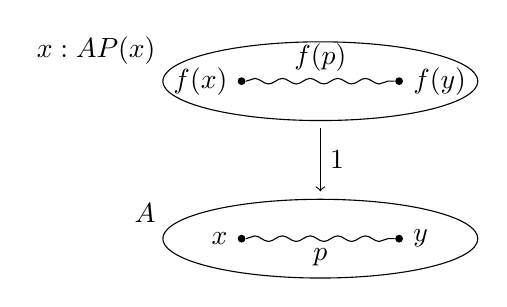
\begin{tikzpicture}[yscale=.5,xscale=2]
    \draw (0,0) arc (-90:170:1cm) node[anchor=south east] {$A$} arc (170:270:1cm);
    \draw (0,4) arc (-90:170:1cm) node[anchor=south east] {$\sm{x:A} P(x)$} arc (170:270:1cm);
    \draw[->] (0,3.8) -- node[auto] {$\proj1$} (0,2.2);
    \node[circle,fill,inner sep=1pt,label=left:{$x$}] (b1) at (-.5,1) {};
    \node[circle,fill,inner sep=1pt,label=right:{$y$}] (b2) at (.5,1) {};
    \draw[decorate,decoration={snake,amplitude=1}] (b1) -- node[auto,swap] {$p$} (b2);
    \node[circle,fill,inner sep=1pt,label=left:{$f(x)$}] (b1) at (-.5,5) {};
    \node[circle,fill,inner sep=1pt,label=right:{$f(y)$}] (b2) at (.5,5) {};
    \draw[decorate,decoration={snake,amplitude=1}] (b1) -- node[auto] {$f(p)$} (b2);
  \end{tikzpicture}
\end{center}

We \emph{can} obtain such a thing from \autoref{lem:map}.
Given $f:\prd{x:A} P(x)$, we can define a non-dependent function $f':A\to \sm{x:A} P(x)$ by setting $f'(x)\defeq (x,f(x))$, and then consider $\ap{f'}{p} : f'(x) = f'(y)$.
However, it is not obvious from the type of such a path that it lies over a specific path in $A$ (in this case, $p$), which is sometimes important.

The solution is to use the transport lemma.
Since there is a canonical path from $u:P(x)$ to $\trans p u :P(y)$ which (at least intuitively) lies over $p$, any path from $u$ to $v:P(y)$ lying over $p$ should factor through this path, essentially uniquely, by a path from $\trans p u$ to $v$ lying entirely in the fiber $P(y)$.
Thus, up to equivalence, it makes sense to define ``a path from $u$ to $v$ lying over $p:x=y$'' to mean a path $\trans p u = v$ in $P(y)$.
And, indeed, we can show that dependent functions produce such paths.

\begin{lem}[Dependent map]\label{lem:mapdep}
  Suppose $f:\prd{x: A} P(x)$; then we have a map
  \[\apdfunc f : \prd{p:x=y}\big(\id[P(y)]{\trans p{f(x)}}{f(y)}\big).\]
\end{lem}

\begin{proof}[First proof]
  Let $D:\prd{x,y:A}{p:\id{x}{y}} \type$ be the type family defined by
  \begin{equation*}
    D(x,y,p)\defeq \trans p {f(x)}= f(y).
  \end{equation*}
  Then $D(x,x,\refl{x})$ is $\trans{(\refl{x})}{f(x)}= f(x)$.
  But since $\trans{(\refl{x})}{f(x)}\jdeq f(x)$, we get that $D(x,x,\refl{x})\jdeq (f(x)= f(x))$.
  Thus, we find the function
  \begin{equation*}
    d\defeq\lam{x} \refl{f(x)}:\prd{x:A} D(x,x,\refl{x})
  \end{equation*}
  and now $J$ gives us $\apdfunc f(p):\trans p{f(x)}= f(y)$ for each $p:x= y$.
\end{proof}

\begin{proof}[Second proof]
  By induction, it suffices to assume $p$ is $\refl x$.
  But in this case, the desired equation is $\trans{(\refl{x})}{f(x)}\jdeq f(x)$, which holds judgmentally.
\end{proof}

We will refer generally to paths which ``lie over other paths'' in this sense as \emph{dependent paths}.
They will play an increasingly important role starting in \autoref{cha:hits}.
In \autoref{sec:computational} we will see that for a few particular kinds of type families, there are equivalent ways to represent the notion of dependent paths that are sometimes more convenient.

Now recall from section \ref{sec:pi-types} that a non-dependently typed function $f:A\to B$ is just the special case of a dependently typed function $f:\prd{x:A} P(x)$ when $P$ is a constant type family, $P(x) \defeq B$.
In this case, $\apdfunc{f}$ and $\apfunc{f}$ are closely related, because of the following lemma:

\begin{lem}\label{thm:trans-trivial}
  If $P:A\to\type$ is defined by $P(x) \defeq B$ for a fixed $B:\type$, then for any $x,y:A$ and $p:x=y$ and $b:B$ we have a path
  \[ \transconst Bpb : \transfib P p b = b. \]
\end{lem}
\begin{proof}[First proof]
  Fix a $b:B$, and let $D:\prd{x,y:A}{p:\id{x}{y}} \type$ be the type family defined by
  \[ D(x,y,p) \defeq (\transfib P p b = b). \]
  Then $D(x,x,\refl x)$ is $(\transfib P{\refl{x}}{b} = b)$, which is judgmentally equal to $(b=b)$ by the computation rule for transporting.
  Thus, we have the function
  \[ d \defeq \lam{x} \refl{b} : \prd{x:A} D(x,x,\refl x). \]
  Now path induction gives us an element of $\prd{x,y:A}{p:x=y}(\transfib P p b = b)$, as desired.
\end{proof}
\begin{proof}[Second proof]
  By induction, it suffices to assume $y$ is $x$ and $p$ is $\refl x$.
  But $\transfib P {\refl x} b \jdeq b$, so in this case what we have to prove is $b=b$, and we have $\refl{b}$ for this.
\end{proof}

Thus, by concatenating with $\transconst B p b$, for any $x,y:A$ and $p:x=y$ and $f:A\to B$ we obtain functions
\begin{align}
  \big(f(x) = f(y)\big) &\to \big(\trans{p}{f(x)} = f(y)\big)\label{eq:ap-to-apd}
  \qquad\text{and} \\
  \big(\trans{p}{f(x)} = f(y)\big) &\to \big(f(x) = f(y)\big).\label{eq:apd-to-ap}
\end{align}
In fact, these functions are inverse equivalences (in the sense to be introduced in \autoref{sec:basics-equivalences}), and they relate $\apfunc f (p)$  to $\apdfunc f (p)$.

\begin{lem}\label{thm:apd-const}
  For $f:A\to B$ and $p:\id[A]xy$, we have
  \[ \apdfunc f(p) = \transconst B p{f(x)} \ct \apfunc f (p) \]
\end{lem}
\begin{proof}[First proof]
  Let $D:\prd{x,y:A}{p:\id xy} \type$ be the type family defined by
  \[ D(x,y,p) \defeq \big(\apdfunc f (p) = \transconst Bp{f(x)} \ct \apfunc f (p)\big). \]
  Thus, we have
  \[D(x,x,\refl x) \jdeq \big(\apdfunc f (\refl x) = \transconst B{\refl x}{f(x)} \ct \apfunc f ({\refl x})\big).\]
  But by definition, all three paths appearing in this type are $\refl{f(x)}$, so we have
  \[ \refl{\refl{f(x)}} : D(x,x,\refl x). \]
  Thus, path induction gives us an element of $\prd{x,y:A}{p:x=y} D(x,y,p)$, which is what we wanted.
\end{proof}
\begin{proof}[Second proof]
  By induction, it suffices to assume $y$ is $x$ and $p$ is $\refl x$.
  In this case, what we have to prove is $\refl{f(x)} = \refl{f(x)} \ct \refl{f(x)}$, which is true judgmentally.
\end{proof}

Because the types of $\apdfunc{f}$ and $\apfunc{f}$ are different, it is often clearer to use different notations for them.
We may sometimes use a notation $\apd f p$ for $\apdfunc{f}(p)$, which is similar to the notation $\ap f p$ for $\apfunc{f}(p)$.

At this point, we hope the reader is starting to get a feel for proofs by induction on identity types.
From now on we stop giving both styles of proofs, allowing ourselves to use whatever is most clear and convenient (and often the second, more concise one).
Here are a few other useful lemmas about transport; we leave it to the reader to give the proofs (in either style).

\begin{lem}\label{thm:transport-concat}
  Given $P:A\to\type$ with $p:\id[A]xy$ and $q:\id[A]yz$ while $u:P(x)$, we have
  \[ \trans{q}{\trans{p}{u}} = \trans{(p\ct q)}{u}. \]
\end{lem}

\begin{lem}\label{thm:transport-compose}
  For a function $f:A\to B$ and a type family $P:B\to\type$, and any $p:\id[A]xy$ and $u:P(f(x))$, we have
  \[ \transfib{P\circ f}{p}{u} = \transfib{P}{\apfunc f(p)}{u}. \]
\end{lem}

\begin{lem}\label{thm:ap-transport}
  For $P,Q:A\to \type$ and a family of functions $f:\prd{x:A} P(x)\to Q(x)$, and any $p:\id[A]xy$ and $u:P(x)$, we have
  \[ \transfib{Q}{p}{f_x(u)} = f_y(\transfib{P}{p}{u}). \]
\end{lem}


\section{Summary of the basic higher structure}
\label{sec:basics-summary}

Here we summarize the basic definitions made in the previous two sections.

\begin{itemize}
\item $\opp{p} : y=x$, for $p:x=y$, defined by
  \[\opp{\;\refl{x}}\jdeq \refl{x}.\]
\item $p\ct q :y=z$, for $p:x=y$ and $q:y=z$, defined by
  \[ \refl{x}\ct\refl{x}\jdeq\refl{x}.\]
\item If $P$ is a type family over $A$ then $\transf{p}:P(x)\to P(y)$, for $p:x=y$, defined by
  \[\transf{(\refl{x})}\jdeq \idfunc[P(x)].\]
\item If $f:A\to B$ then $\map{f}{p}:f(x)=f(y)$, for $p:x=y$, defined by
  \[\map{f}{\refl{x}}\jdeq \refl{f(x)}.\]
\item If $f:\prod_{x:A}P(x)$ then $\mapdep{f}{p}:\trans{p}{f(x)}=f(y)$, for $p:x=y$, defined by
  \[\mapdep{f}{\refl{x}}\jdeq \refl{f(x)}.\]
\end{itemize}


\section{Homotopies and equivalences}
\label{sec:basics-equivalences}

So far, we have seen how the identity type $\id[A]xy$ can be regarded as a type of \emph{identifications}, \emph{paths}, or \emph{equivalences} between two elements $x$ and $y$ of a type $A$.
Now we investigate the appropriate notions of ``identification'' or ``sameness'' between \emph{functions} and between \emph{types}.
In \S\ref{sec:computational}, we will see that homotopy type theory allows us to identify these with instances of the identity type, but before we can do that we need to understand them in their own right.

Traditionally, we regard two functions as the same if they take equal values on all inputs.
Under the propositions-as-types interpretation, this suggests that two functions $f$ and $g$ should be the same if the type $\prd{x:A} (f(x)=g(x))$ is inhabited.
Under the homotopical interpretation, this dependent function type consists of \emph{continuous} paths or \emph{functorial} equivalences, and thus may be regarded as the type of \emph{homotopies} or of \emph{natural isomorphisms}.
We will adopt the topological terminology for this.
Note that it makes perfect sense even when $f$ and $g$ are dependent functions.

\begin{defn}
  Let $f,g:\prd{x:A} P(x)$ be two sections of a type family $P:A\to\type$.
  A \textbf{homotopy} from $f$ to $g$ is a term of type
  \begin{equation*}
    (f\htpy g)\;\defeq\; \prd{x:A} (f(x)=g(x))
  \end{equation*}
\end{defn}

Note that a homotopy is not the same as an identification $(f=g)$.
In \S\ref{sec:compute-pi} we will show that homotopies and identifications are nevertheless ``equivalent''.

The following proofs are left to the reader.

\begin{lem}\label{lem:homotopy-props}
  Homotopy is an equivalence relation on each function type $A\ra B$.
  That is, we have elements of the types
  \begin{gather*}
    \prd{f:A\to B} (f\htpy f)\\
    \prd{f,g:A\to B} (f\htpy g) \to (g\htpy f)\\
    \prd{f,g,h:A\to B} (f\htpy g) \to (g\htpy h) \to (f\htpy h).
  \end{gather*}
\end{lem}

\begin{lem}
  Composition is associative and unital up to homotopy.
  That is:
  \begin{enumerate}
  \item If $f:A\ra B$ then $f\circ \idfunc[A]\htpy f\htpy \idfunc[B]\circ f$.
  \item If $f:A\ra B, g:B\ra C$ and $h:C\ra D$ then $h\circ (g\circ f)\;\htpy\; (h\circ g)\circ f$.
  \end{enumerate}
\end{lem}

The first level of the continuity/naturality of homotopies can be expressed as follows:

\begin{lem}\label{lem:htpy_natural}
  Suppose $H:f\htpy g$ is a homotopy between functions $f,g:A\to B$ and let $p:\id[A]xy$.  Then there is a term of type
  \begin{equation*}
    H(x)\ct\ap{g}{p}=\ap{f}{p}\ct H(y).
  \end{equation*}
  We may also draw this as a commutative diagram:
  \begin{align*}
    \xymatrix{
      f(x) \ar[r]^{\ap fp} \ar[d]_{H(x)} & f(y) \ar[d]^{H(y)} \\
      g(x) \ar[r]_{\ap gp} & g(y)
    }
  \end{align*}
\end{lem}
\begin{proof}
  By induction, we may assume $p$ is $\refl x$.
  Since $\apfunc{f}$ and $\apfunc g$ compute on reflexivity, in this case what we must show is
  \[ H(x) \ct \refl{g(x)} = \refl{f(x)} \ct H(x). \]
  But this follows since both sides are equal to $H(x)$.
\end{proof}

\newcommand{\com}[3]{\mathtt{swap}_{#1,#2}(#3)}
\begin{cor}\label{cor:hom-fg}
Let $H : f \htpy \idfunc[A]$ be a homotopy, with $f : A \to A$. Then for any $x : A$ we have \[ H(f(x)) = \ap f{H(x)}. \] The above path will be denoted by $\com{h}{f}{x}$.
\end{cor}
\begin{proof}
By naturality of $H$, the following diagram commutes:
\begin{align*}
\xymatrix{
ffx \ar[r]^{\ap f{Hx}} \ar[d]_{H(fx)} & fx \ar[d]^{Hx} \\
fx \ar[r]_{Hx} & x
}
\end{align*}
Canceling $H(x)$, we see that $h(fx) = f(hx)$ as desired.
\end{proof}

Moving on to types, from a traditional perspective one may say that a function $f:A\to B$ is an \emph{isomorphism} if there is a function $g:B\to A$ such that both composites $f\circ g$ and $g\circ f$ are pointwise equal to the identity, i.e.\ such that $f \circ g \htpy \idfunc[B]$ and $g\circ f \htpy \idfunc[A]$.
A homotopical perspective suggests that this should be called a \emph{homotopy equivalence}, and from a categorical one, it should be called an \emph{equivalence of (higher) groupoids}.
However, when doing proof-relevant mathematics, the corresponding type
\begin{equation}
  \sm{g:B\to A} \big((f \circ g \htpy \idfunc[B]) \times (g\circ f \htpy \idfunc[A])\big)\label{eq:qinvtype}
\end{equation}
is poorly behaved.
For instance, for a single function $f:A\to B$ there may be multiple inhabitants of~\eqref{eq:qinvtype} which are not provably equal.
(This is closely related to the observation in higher category theory that often one needs to consider \emph{adjoint} equivalences rather than plain equivalences.)
For this reason, we give~\eqref{eq:qinvtype} the following historically accurate, but slightly derogatory-sounding name instead.

\begin{defn}
  For a function $f:A\to B$, a \textbf{quasi-inverse} of $f$ is a triple $(g,\alpha,\beta)$ consisting of a function $g:B\to A$ and homotopies
$\alpha:f\circ g\htpy \idfunc[B]$ and $\beta:g\circ f\htpy \idfunc[A]$.
\end{defn}

Thus,~\eqref{eq:qinvtype} is \emph{the type of quasi-inverses of $f$}; we may denote it by $\qinv(f)$.

\begin{eg}\label{eg:idequiv}
  The identity function $\idfunc[A]:A\to A$ has a quasi-inverse given by $\idfunc[A]$ itself, together with homotopies defined by $\alpha(y) \defeq \refl{y}$ and $\beta(x) \defeq \refl{x}$.
\end{eg}

In general, we will only use the word \emph{isomorphism} (and similar words such as \emph{bijection}) in the special case when the types $A$ and $B$ ``behave like sets'' (see \S\ref{sec:basics-sets}).
In this case, the type~\eqref{eq:qinvtype} is unproblematic.
We will reserve the word \emph{equivalence} for an improved notion with the following properties:
\begin{enumerate}
\item For each $f:A\to B$ there is a function $\qinv(f) \to \isequiv (f)$.\label{item:be1}
\item Similarly, for each $f$ we have $\isequiv (f) \to \qinv(f)$; thus the two are ``logically equivalent''.\label{item:be2}
\item For any two inhabitants $e_1,e_2:\isequiv(f)$ we have $e_1=e_2$.\label{item:be3}
\end{enumerate}
In Chapter~\ref{cha:equivalences} we will see that there are many different definitions of $\isequiv(f)$ which satisfy these three properties, but that all of them are equivalent.
For now, to convince the reader that such things exist, we mention only the easiest such definition (though it is not the one we will eventually settle on in Chapter~\ref{cha:equivalences}):
\begin{equation}
  \isequiv(f) \;\defeq\;
  \big(\sm{g:B\to A} (f\circ g \htpy \idfunc[B])\big)
  \times
  \big(\sm{h:B\to A} (h\circ f \htpy \idfunc[A])\big)\label{eq:isequiv-invertible}
\end{equation}
We can show~\ref{item:be1} and~\ref{item:be2} for this definition now.
A function $\qinv(f) \to \isequiv (f)$ is easy to define by taking $(g,\alpha,\beta)$ to $(g,\alpha,g,\beta)$.
In the other direction, given $(g,\alpha,h,\beta)$, let $\gamma$ be the composite homotopy
\[ g \overset{\beta}{\htpy} h\circ f\circ g \overset{\alpha}{\htpy} h \]
and let $\beta':g\circ f\htpy \idfunc[A]$ be obtained from $\gamma$ and $\beta$.
Then $(g,\alpha,\beta'):\qinv(f)$.

Property~\ref{item:be3} for this definition is not too hard to prove either, but it requires identifying the identity types of cartesian products and dependent pair types, which we will discuss in \S\ref{sec:computational}.
Thus, we postpone it as well.
At this point, the main thing to take away is that there is a well-behaved type which we can pronounce as ``$f$ is an equivalence'', and that we can prove $f$ to be an equivalence by exhibiting a quasi-inverse to it.
In practice, this is the most common approach.

In accord with the proof-relevant philosophy, \emph{an equivalence} from $A$ to $B$ is defined to be a function $f:A\to B$ together with an inhabitant of $\isequiv (f)$, i.e.\ a proof that it is an equivalence.
We write $(\eqv A B)$ for the type of equivalences from $A$ to $B$, i.e.\ the type
\[ (\eqv A B) \;\defeq \; \sm{f:A\to B} \isequiv(f). \]
Property~\ref{item:be3} above will ensure that if two equivalences are equal as functions (that is, the underlying elements of $A\to B$ are equal), then they are also equal as equivalences (see \S\ref{sec:compute-sigma}).

% Local Variables:
% TeX-master: "main"
% End:


\newcommand{\fcomp}{\circ}

\section{The computational behavior of type formers}
\label{sec:computational}

In \autoref{cha:typetheory}, we introduced many ways to form new types: cartesian products, disjoint unions, dependent products, dependent sums, etc.
In the previous sections of this chapter, we have seen that \emph{all} types in homotopy type theory behave like spaces or higher groupoids.
Our goal in this section is to make explicit how this higher structure behaves, for particular types defined as in \autoref{cha:typetheory}.

It turns out that for many types $A$, the equality types $\id[A]xy$ can be characterized, up to equivalence, in terms of whatever data was used to construct $A$.
For instance, if $A$ is a cartesian product $B\times C$, and $x\jdeq (b,c)$ and $y\jdeq(b',c')$, then we have an equivalence
\begin{equation}\label{eq:prodeqv}
  \eqv{\Big((b,c)=(b',c')\Big)}{\Big((b=b')\times (c=c')\Big)}.
\end{equation}
In more traditional language, two ordered pairs are equal just when their components are equal (but the equivalence~\eqref{eq:prodeqv} says rather more than this).
The higher structure of the identity types can also be expressed in terms of these equivalences; for instance, concatenating two equalities between pairs corresponds to pairwise concatenation.

Similarly, when a type family $P:A\to\type$ is built up fiberwise using the type forming rules from \autoref{cha:typetheory}, the operation $\transfib{P}{p}{-}$ can be characterized, up to homotopy, in terms of the corresponding operations on the data that went into $P$.
For instance, if $P(x) \jdeq B(x)\times C(x)$, then we have
\[\transfib{P}{p}{(b,c)} = \left(\transfib{B}{p}{b},\transfib{C}{p}{c}\right).\]

Finally, the type forming rules are also functorial, and if a function $f$ is built from this functoriality, then the operations $\apfunc f$ and $\apdfunc f$ can be computed based on the corresponding ones on the data going into $f$.
For instance, if $g:B\to B'$ and $h:C\to C'$ and we define $f:B\times C \to B'\times C'$ by $f(b,c)\defeq (g(b),h(c))$, then modulo the equivalence~\eqref{eq:prodeqv}, we can identify $\apfunc f$ with ``$(\apfunc g,\apfunc h)$''.

In this section, we will state and prove theorems of this sort for all the basic type forming rules.

\begin{rmk}\label{rmk:computational-hope}
  In the type theory we are working with, identity types are defined simultaneously for all types by their induction principle.
  The characterizations for particular types to be discussed in this chapter are then theorems which we have to discover and prove.
  An alternative presentation of type theory might take these characterizations as \emph{definitions} of the identity types (by induction over the construction of types), with the general induction principle then being provable.
  While such a type theory has not yet been made precise except in very simple cases, it is still helpful to think of the rules to be presented in this section as ``computation'' rules for ``evaluating'' identity types, transport, and function application.
  It is important to note, though, that not \emph{all} identity types can be ``defined'' by induction over the construction of types; counterexamples include most nontrivial higher inductive types (see \autoref{cha:hits,cha:homotopy}).
\end{rmk}

\subsection{Cartesian product types}
\label{sec:compute-cartprod}

Given types $A$ and $B$, consider the cartesian product type $A \times B$.  
For any elements $x,y:A\times B$ and a path $p:\id[A\times B]{x}{y}$, by functoriality we can extract paths $\ap{\proj1}p:\id[A]{\proj1(x)}{\proj1(y)}$ and $\ap{\proj2}p:\id[B]{\proj2(x)}{\proj2(y)}$.
Thus, we have a function
\begin{equation}
  (\id[A\times B]{x}{y}) \;\to\; (\id[A]{\proj1(x)}{\proj1(y)}) \times (\id[B]{\proj2(x)}{\proj2(y)}).\label{eq:path-prod}
\end{equation}

\begin{thm}\label{thm:path-prod}
  For any $x$ and $y$, the function~\eqref{eq:path-prod} is an equivalence.
\end{thm}

Read logically, this says that two pairs are equal if they are equal
componentwise.  Read category-theoretically, this says that the
morphisms in a product groupoid are pairs of morphisms.  Read
homotopy-theoretically, this says that the paths in a product
space are pairs of paths.

\begin{proof}
  We need a function in the other direction:
  \begin{equation}
    (\id[A]{\proj1(x)}{\proj1(y)}) \times (\id[B]{\proj2(x)}{\proj2(y)}) \;\to\; (\id[A\times B]{x}{y}) .\label{eq:path-prod-inverse}
  \end{equation}
  By the induction rule for cartesian products, we may assume that $x$ and $y$ are both pairs, i.e.\ $x\jdeq (a,b)$ and $y\jdeq (a',b')$ for some $a,a':A$ and $b,b':B$.
  In this case, what we want is a function
  \begin{equation*}
    (\id[A]{a}{a'}) \times (\id[B]{b}{b'}) \;\to\; \big(\id[A\times B]{(a,b)}{(a',b')}\big).
  \end{equation*}
  Now by induction for the cartesian product in its domain, we may assume given $p:a=a'$ and $q:b=b'$.
  And by two path inductions, we may assume that $a\jdeq a'$ and $b\jdeq b'$ and both $p$ and $q$ are reflexivity.
  But in this case, we have $(a,b)\jdeq(a',b')$ and so we can take the output to also be reflexivity.

  It remains to prove that~\eqref{eq:path-prod-inverse} is quasi-inverse to~\eqref{eq:path-prod}.
  This is a simple sequence of inductions, but they have to be done in the right order.

  In one direction, let us start with $r:\id[A\times B]{x}{y}$.
  We first do a path induction on $r$ in order to assume that $x\jdeq y$ and $r$ is reflexivity.
  In this case, since $\apfunc{\proj1}$ and $\apfunc{\proj2}$ are defined by path induction,~\eqref{eq:path-prod} takes $r\jdeq \refl{x}$ to the pair $(\refl{\proj1x},\refl{\proj2x})$.
  Now by induction on $x$, we may assume $x\jdeq (a,b)$, so that this is $(\refl a, \refl b)$.
  Thus,~\eqref{eq:path-prod-inverse} takes it by definition to $\refl{(a,b)}$, which (under our current assumptions) is $r$.
  
  In the other direction, if we start with $s:(\id[A]{\proj1(x)}{\proj1(y)}) \times (\id[B]{\proj2(x)}{\proj2(y)})$, then we first do induction on $x$ and $y$ to assume that they are pairs $(a,b)$ and $(a',b')$, and then induction on $s:(\id[A]{a}{a'}) \times (\id[B]{b}{b'})$ to reduce it to a pair $(p,q)$ where $p:a=a'$ and $q:b=b'$.
  Now by induction on $p$ and $q$, we may assume they are reflexivities $\refl a$ and $\refl b$, in which case~\eqref{eq:path-prod-inverse} yields $\refl{(a,b)}$ and then~\eqref{eq:path-prod} returns us to $(\refl a,\refl b)\jdeq (p,q)\jdeq s$.
\end{proof}

In particular, we have shown that~\eqref{eq:path-prod} has an inverse~\eqref{eq:path-prod-inverse}, which we may denote by
\[
\pairpath : (\id{\proj{1}(x)}{\proj{1}(y)}) \times (\id{\proj{1}(x)}{\proj{1}(y)}) \;\to\; {(\id x y)}
\]
Note that a special case of this yields the $\eta$-equivalence rule for products: $z = (\proj1(z),\proj2(z))$.

It can be helpful to view \pairpath as a \emph{constructor} or \emph{introduction rule} for $\id x y$, analogous to the ``pairing'' constructor of $A\times B$ itself, which introduces the pair $(a,b)$ given $a:A$ and $b:B$.
From this perspective, the two components of~\eqref{eq:path-prod}:
\begin{align*}
  \projpath{1} &: (\id{x}{y}) \to (\id{\proj{1}(x)}{\proj{1} (y)})\\
  \projpath{2} &: (\id{x}{y}) \to (\id{\proj{2}(x)}{\proj{2} (y)})
\end{align*}
are \emph{elimination} rules.
Similarly, the two homotopies which witness~\eqref{eq:path-prod-inverse} as quasi-inverse to~\eqref{eq:path-prod} consist respectively, of \emph{computation} or \emph{$\beta$-reduction} rules:
\begin{align*}
  {\projpath{1}{(\pairpath(p, q)})}
  &= %_{(\id{\proj{1} x}{\proj{1} y})}
  {p} \qquad\text{for } p:\id{\proj{1} x}{\proj{1} y} \\
  {\projpath{2}{(\pairpath(p,q)})}
  &= %_{(\id{\proj{2} x}{\proj{2} y})}
  {q} \qquad\text{for } q:\id{\proj{2} x}{\proj{2} y}
\end{align*}
and an \emph{$\eta$-equivalence} rule:
\[
\id{r}{\pairpath(\projpath{1} (r), \projpath{2} (r)) }
\qquad\text{for } r : \id[A \times B] x y
\]

We can also characterize the reflexivity, inverses, and composition of paths in $A\times B$ componentwise:
\begin{align*}
  {\refl{(z : A \times B)}}
  &= {\pairpath (\refl{\proj{1} z},\refl{\proj{2} z})} \\
  {\opp{p}}
  &= {\pairpath \big(\opp{\projpath{1} (p)},\, \opp{\projpath{2} (p)}\big)} \\
  {{p \ct q}}
  &= {\pairpath \big({\projpath{1} (p)} \ct {\projpath{1} (q)},\,{\projpath{2} (p)} \ct {\projpath{2} (q)}\big)}
\end{align*}
The same is true for the rest of the higher groupoid structure considered in \autoref{sec:equality}.
All of these equations can be derived by using path induction on the given paths and then returning reflexivity.  

We now consider transport in a pointwise product of type families.
Given type families $ A, B : Z \to \type$, we abusively write $A\times B:Z\to \type$ for the type family defined by $(A\times B)(z) \defeq A(z) \times B(z)$.
Now given $p : \id[Z]{z}{w}$ and $x : A(z) \times B(z)$, we can transport $x$ along $p$ to obtain an element of $A(w)\times B(w)$.

\begin{thm}\label{thm:trans-prod}
  In the above situation, we have
  \[
  \id[A(y) \times B(y)]
  {\transfib{A\times B}px}
  {(\transfib{A}{p}{\proj{1}x}, \transfib{B}{p}{\proj{2}x})}
  \]
\end{thm}
\begin{proof}
  By path induction, we may assume $p$ is reflexivity, in which case we have
  \begin{align*}
    \transfib{A\times B}px&\jdeq x\\
    \transfib{A}{p}{\proj{1}x}&\jdeq \proj1x\\
    \transfib{A}{p}{\proj{2}x}&\jdeq \proj2x.
  \end{align*}
  Thus, it remains to show $x = (\proj1 x, \proj2x)$.
  But this is $\eta$-equivalence, which as we remarked above follows from \autoref{thm:path-prod}.
\end{proof}

Finally, we consider the functoriality of $\apfunc{}$ under cartesian products.
Suppose given types $A,B,A',B'$ and functions $g:A\to A'$ and $h:B\to B'$; then we can define a function $f:A\times B\to A'\times B'$ by $f(x) \defeq (g(\proj1x),h(\proj2x))$.

\begin{thm}\label{thm:ap-prod}
  In the above situation, given $x,y:A\times B$ and $p:\proj1x=\proj1y$ and $q:\proj2x=\proj2y$, we have
  \[ \id[(f(x)=f(y))]{\ap{f}{\pairpath(p,q)}} {\pairpath(\ap{g}{p},\ap{h}{q})}. \]
\end{thm}
\begin{proof}
  Note first that the above equation is well-typed.
  On the one hand, since $\pairpath(p,q):x=y$ we have $\ap{f}{\pairpath(p,q)}:f(x)=f(y)$.
  On the other hand, since $\proj1(f(x))\jdeq g(\proj1x)$ and $\proj2(f(x))\jdeq h(\proj2x)$, we also have $\pairpath(\ap{g}{p},\ap{h}{q}):f(x)=f(y)$.

  Now, by induction, we may assume $x\jdeq(a,b)$ and $y\jdeq(a',b')$, in which case we have $p:a=a'$ and $q:b=b'$.
  Thus, by path induction, we may assume $p$ and $q$ are reflexivity, in which case the desired equation holds judgmentally.
\end{proof}


\subsection{\texorpdfstring{$\Sigma$}{Σ}-types}
\label{sec:compute-sigma}

Let $A$ be a type and $B:A\to\type$ a type family.
Recall that the $\Sigma$-type, or dependent pair type, $\sm{x:A} B(x)$ is a generalization of the cartesian product type.
Thus, we expect its higher groupoid structure to also be a generalization of the previous section.
In particular, its paths should be pairs of paths, but it takes a little thought to give the correct types of these paths.

Suppose that we have a path $p:w=w'$ in $\sm{x:A}P(x)$.
Then we get $\ap{\proj{1}}{p}:\proj{1}(w)=\proj{1}(w')$.
However, we cannot directly ask whether $\proj{2}(w)$ is identical to $\proj{2}(w')$ since they don't have to be in the same type.
But we can transport $\proj{2}(w)$ along the path $\ap{\proj{1}}{p}$, and this does give us an element of the same type as $\proj{2}(w')$.
By path induction, we do in fact obtain a path $\trans{\ap{\proj{1}}{p}}{\proj{2}(w)}=\proj{2}(w')$.

Recall from the discussion preceeding \autoref{lem:mapdep} that $\trans{\ap{\proj{1}}{p}}{\proj{2}(w)}=\proj{2}(w')$ can be regarded as the type of paths from $\proj2(w)$ to $\proj2(w')$ which lie over the path $\ap{\proj1}{p}$ in $A$.
Thus, we are saying that a path $w=w'$ in the total space determines (and is determined by) a path $p:\proj1(w)=\proj1(w')$ in $A$ together with a path from $\proj2(w)$ to $\proj2(w')$ lying over $p$, which seems sensible.

\begin{rmk}
  Note that if we have $x:A$ and $u,v:P(x)$ such that $(x,u)=(x,v)$, it does not follow that $u=v$.
  All we can conclude is that there exists $p:x=x$ such that $\trans p u = v$.
  This is a well-known source of confusion for newcomers to type theory, but it makes sense from a topological viewpoint: the existence of a path $(x,u)=(x,v)$ in the total space of a fibration betweeen two points that happen to lie in the same fiber does not imply the existence of a path $u=v$ lying entirely \emph{within} that fiber.
\end{rmk}

The next theorem states that we can also reverse this process.
Since it is a direct generalization of \autoref{thm:path-prod}, we will be more concise.

\begin{thm}\label{thm:path-sigma}
Suppose that $P:A\to\type$ is a type family over a type $A$ and let $w,w^\prime:\sm{x:A}P(x)$. Then there is an equivalence
\begin{equation*}
\eqvspaced{(w=w')}{\dsm{p:\proj{1}(w)=\proj{1}(w')} \trans{p}{\proj{2}(w)}=\proj{2}(w^\prime)}.
\end{equation*}
\end{thm}

\begin{proof}
We define for any $w,w':\sm{x:A}P(x)$, a function
\begin{equation*}
f: (w=w') \;\to\; \dsm{p:\proj{1}(w)=\proj{1}(w')} \trans{p}{\proj{2}(w)}=\proj{2}(w^\prime)
\end{equation*}
by path induction, with
\begin{equation*}
f(w,w,\refl{w})\defeq(\refl{\proj{1}(w)},\refl{\proj{2}(w)}).
\end{equation*}
We want to show that $f$ is an equivalence.

In the reverse direction, we define
\begin{equation*}
  g : \dprd{w,w':\sm{x:A}P(x)} \left(\dsm{p:\proj{1}(w)=\proj{1}(w')}\trans{p}{\proj{2}(w)}=\proj{2}(w^\prime)\right)
  \;\to\; (w=w')
\end{equation*}
by first inducting on $w$ and $w'$, which splits them into $(w_1,w_2)$ and
$(w_1',w_2')$ respectively, so it suffices to show 
\begin{equation*}
\left(\dsm{p:w_1 = w_1'}\trans{p}{w_2}=w_2^\prime\right) \;\to\; ((w_1,w_2)=(w_1',w_2'))
\end{equation*}
Next, given a pair $\sm{p:w_1 = w_1'}\trans{p}{w_2}=w_2^\prime$, we can
use $\Sigma$-induction to get $p : w_1 = w_1'$ and $q :
\trans{p}{w_2}=w_2^\prime$.  Inducting on $p$, we have $q :
\trans{\refl{}}{w_2}=w_2^\prime$, and it suffices to show 
$(w_1,w_2)=(w_1,w_2')$.  But $\trans{\refl{}}{w_2} \jdeq w_2$, so
inducting on $q$ reduces to the goal to 
$(w_1,w_2)=(w_1,w_2)$, which we can prove with $\refl{(w_1,w_2)}$.  

Next we show that $f \circ g$ is the identity for all $w$, $w'$ and
$r$, where $r$ has type
\[\dsm{p:\proj{1}(w)=\proj{1}(w')} (\trans{p}{\proj{2}(w)}=\proj{2}(w^\prime)).\]
First, we break apart the pairs $w$, $w'$, and $r$ by pair induction, as in the
definition of $g$, and then use two path inductions to reduce both components
of $r$ to \refl{}.  Then it suffices to show that 
$f (g(\refl{},\refl{})) = \refl{}$, which is true by definition.

Similarly, to show that $g \circ f$ is the identity for all $w$, $w'$,
and $p : w = w'$, we can do path-induction $p$, and then induction to
split $w$, at which point it suffices to show that
$g(f (\refl{(w_1,w_2)})) = \refl{(w_1,w_2)}$, which is true by
definition.

Thus, $f$ has a quasi-inverse, and is therefore an equivalence.  
\end{proof}

As we did in the case of cartesian products, we have $\eta$-equivalence as a special case.

\begin{cor}\label{thm:eta-sigma}
  For $z:\sm{x:A} P(x)$, we have $z = (\proj1(z),\proj2(z))$.
\end{cor}
\begin{proof}
  We have $\refl{\proj1(z)} : \proj1(z) = \proj1(\proj1(z),\proj2(z))$, so by \autoref{thm:path-sigma} it will suffice to exhibit a path $\trans{(\refl{\proj1(z)})}{\proj2(z)} = \proj2(\proj1(z),\proj2(z))$.
  But both sides are judgmentally equal to $\proj2(z)$.
\end{proof}

Like with binary cartesian products, we can think of 
the backward direction of \autoref{thm:path-sigma} as
an introduction form (\pairpath{}{}), the forward direction as
elimination forms (\projpath{1} and \projpath{2}), and the equivalence
as giving $\beta$ and $\eta$ rules for these.  

Note that the lifted path $\mathsf{lift}(u,p)$  of $p:x=y$ at $u:P(x)$ defined in \autoref{thm:path-lifting} may be identified with the special case of the introduction form
\[\pairpath(p,\refl{\trans p u}):(x,u) = (y,\trans p u).\]
This appears in the statement of action of transport on $\Sigma$-types, which is also a generalization of the action for binary cartesian products:

\begin{thm}
  Suppose we have type families $P:A\to\type$ and $Q:\big(\sm{x:A} P(x)\big)\to\type$.
  Then we can construct the type family over $A$ defined by
  \begin{equation*}
    x \;\mapsto\;  \sm{u:P(x)} Q(x,u).
  \end{equation*}
  For any path $p:x=y$ and any $(u,z):\sum(u:P(x)),\ Q(x,u)$ we have
  \begin{equation*}
    \trans{p}{u,z}=\big(\trans{p}{u},\,\trans{\pairpath(p,\refl{\trans pu})}{z}\big).
  \end{equation*}
\end{thm}

\begin{proof}
Immediate by path induction.
\end{proof}

We leave it to the reader to state and prove a generalization of
\autoref{thm:ap-prod} (see \autoref{ex:ap-sigma}), and to characterize
the reflexivity, inverses, and composition of $\Sigma$-types
componentwise.


\subsection{The unit type}
\label{sec:compute-unit}

Trivial cases are sometimes important, so we mention briefly the case of the unit type \unit.

\begin{thm}\label{thm:path-unit}
  For any $x,y:\unit$, we have $\eqv{(x=y)}{\unit}$.
\end{thm}
\begin{proof}
  A function $(x=y)\to\unit$ is easy to define by sending everything to \ttt.
  Conversely, for any $x,y:\unit$ we may assume by induction that $x\jdeq \ttt\jdeq y$.
  In this case we have $\refl{\ttt}:x=y$, yielding a constant function $\unit\to(x=y)$.

  To show that these are inverses, consider first an element $u:\unit$.
  We may assume that $u\jdeq\ttt$, but this is also the result of the composite $\unit \to (x=y)\to\unit$.

  On the other hand, suppose given $p:x=y$.
  By path induction, we may assume $x\jdeq y$ and $p$ is $\refl x$.
  We may then assume that $x$ is \ttt, in which case the composite $(x=y) \to \unit\to(x=y)$ takes $p$ to $\refl x$, i.e.\ to $p$.
\end{proof}

In particular, any two elements of $\unit$ are equal.
We leave it to the reader to formulate this equivalence in terms of introduction, elimination, $\beta$, and $\eta$ rules.
The transport lemma for \unit is simply the transport lemma for constant type families.


\subsection{\texorpdfstring{$\Pi$}{Π}-types}
\label{sec:compute-pi}

Given a type $A$ and a type family $B : A \to \type$, consider the dependent function type $\prd{x:A}B(x)$.
We expect paths $f=g$ in $\prd{x:A} B(x)$ to be equivalent to pointwise paths:
\begin{equation}
  \eqvspaced{(\id{f}{g})}{\big(\prd{x:A} (\id[B(x)]{f(x)}{g(x)})\big)}\label{eq:path-forall}
\end{equation}
From a traditional perspective, this would say that two functions which are equal at each point are equal as functions.
From a topological perspective, it would say that a path in a function space is the same as a continuous homotopy.
And from a categorical perspective, it would say that an isomorphism in a functor category is a natural family of isomorphisms.

Unlike the case in the previous sections, however, the basic type theory presented in \autoref{cha:typetheory} is insufficient to prove~\eqref{eq:path-forall}.
All we can say is that there is a function
\begin{equation}
  \happly : {(\id{f}{g})}\;\to\; \prd{x:A} (\id[B(x)]{f(x)}{g(x)})\label{eq:happly}
\end{equation}
which is easily defined by path induction.
For the moment, therefore, we will assume:

\begin{axiom}[Function extensionality]\label{axiom:funext}
  For any $A$, $B$, $f$, and $g$, the function~\eqref{eq:happly} is an equivalence.
\end{axiom}

We will see in later chapters that this axiom follows both from univalence (see \autoref{sec:compute-universe} and \autoref{cha:univalence}) and from an interval type (see \autoref{sec:interval}).
Moreover, it could be more naturally built into a computational version of homotopy type theory, as envisioned in \autoref{rmk:computational-hope}.

In particular,~\eqref{eq:happly} has a quasi-inverse
\[
\funext : \left(\prd{x:A} (\id{f(x)}{g(x)})\right) \to {(\id{f}{g})}
\]
which is also called ``function extensionality''.
As we did with $\pairpath$ in \autoref{sec:compute-cartprod}, we can regard $\funext$ as an \emph{introduction rule} for the type $\id f g$.
From this point of view, $\happly$ is the \emph{elimination rule}, while the homotopies witnessing $\funext$ as quasi-inverse to $\happly$ become a $\beta$-reduction rule
\[
\id{\happly({\funext{(h)}},x)}{h(x)} \qquad\text{for }h:\prd{x:A} (\id{f(x)}{g(x)})
\]
and an $\eta$-equivalence rule:
\[
\id{p}{\funext (x \mapsto \happly(p,{x}))} \qquad\text{for } p: (\id f g)
\]
%% FIXME: where do the rules for \alpha[\delta] go in this style?

We can also compute the identity, inverses, and composition in $\Pi$-types; they are simply given by pointwise operations.
\begin{align*}
\refl{f} &= \funext(x \mapsto \refl{f(x)}) \\
\opp{\alpha} &= \funext (x \mapsto \opp{\happly (\alpha)(x)})  \\
{\alpha} \ct \beta &= \funext (x \mapsto {\happly({\alpha})(x) \ct \happly({\beta})(x)})
\end{align*}

Since the non-dependent function type $A\to B$ is a special case of the dependent function type $\prd{x:A} B(x)$ when $B$ is independent of $x$, everything we have said above applies in non-dependent cases as well.
The rules for transport, however, are somewhat simpler in the non-dependent case.
Given a type $X$, a path $p:\id[X]{x_1}{x_2}$, type families $A,B:X\to \type$, and a function $f : A(x_1) \to B(x_1)$,  we have
\begin{align}\label{eq:transport-arrow}
  \transfib{A\to B}{p}{f} &=
  \; \Big(x \mapsto \transfib{B}{p}{f(\transfib{A}{\opp p}{x})}\Big)
\end{align}
where $A\to B$ denotes abusively the type family $X\to \type$ defined by
\[(A\to B)(x) \defeq (A(x)\to B(x)).\]
In other words, when we transport a function $f:A(x_1)\to B(x_1)$ along a path $p:x_1=x_2$, we obtain the function $A(x_2)\to B(x_2)$ which transports its argument backwards along $p$ (in the type family $A$), applies $f$, and then transports the result forwards along $p$ (in the type family $B$).
This can be proven easily by path induction.

Transporting dependent functions is similar, but more complicated.
Suppose given $X$ and $p$ as before, type families $A:X\to \type$ and $B:\prd{x:X} (A(x)\to\type)$, and also a dependent function $f : \prd{a:A(x_1)} B(x_1,a)$.
Then for $p:\id[A]{x_1}{x_2}$ and $a:A(x_2)$, we have
\begin{align*}
  \transfib{\Pi_A(B)}{p}{f}(a) =
  \Transfib{\hat{B}}{\opp{(\pairpath(\opp{p},\refl{ \trans{\opp p}{a} }))}}{f(\transfib{A}{\opp p}{a})}
\end{align*}
where $\Pi_A(B)$ and $\hat{B}$ denote respectively the type families
\begin{equation}\label{eq:transport-arrow-families}
\begin{array}{rclcl}
\Pi_A(B) &\defeq& \big(x\mapsto \prd{a:A(x)} B(x,a) \big) &:& X\to \type\\
\hat{B} &\defeq& \big(w \mapsto B(\proj1w,\proj2w) \big) &:& \big(\sm{x:X} A(x)\big) \to \type.
\end{array}
\end{equation}
If these formulas look a bit intimidating, don't worry about the details.
The basic idea is just the same as for the non-dependent function type: we transport the argument backwards, apply the function, and then transport the result forwards again.

Now recall that for a general type family $P:X\to\type$, in \autoref{sec:functors} we defined the type of \emph{dependent paths} over $p:\id[X]xy$ from $u:P(x)$ to $v:P(y)$ to be $\id[P(y)]{\trans{p}{u}}{v}$.
When $P$ is a family of function types, there is an equivalent way to represent this which is often more convenient.

\begin{lem}\label{thm:dpath-arrow}
  Given type families $A,B:X\to\type$ and $p:\id[X]xy$, and also $f:A(x)\to B(x)$ and $g:A(y)\to B(y)$, we have an equivalence
  \[ \eqvspaced{ \big(\trans{p}{f} = {g}\big) } { \prd{a:A(x)}  (\trans{p}{f(a)} = g(\trans{p}{a})) }. \]
  Moreover, if $q:\trans{p}{f} = {g}$ corresponds under this equivalence to $\hat q$, then for $a:A(x)$, the path
  \[ \happly(q,\trans p a) : (\trans p f)(\trans p a) = g(\trans p a)\]
  is equal to the composite
  \begin{alignat*}{2}
    (\trans p f)(\trans p a)
    &= \trans p {f (\trans {\opp p}{\trans p a})}
    &&\quad\text{by~\eqref{eq:transport-arrow}}\\
    &= \trans p {f(a)}\\
    &= g(\trans p a)
    &&\quad\text{by $\hat{q}$.}
  \end{alignat*}
\end{lem}
\begin{proof}
  By path induction, we may assume $p$ is reflexivity, in which case the desired equivalence reduces to function extensionality.
  The second statement then follows by the computation rule for function extensionality.
\end{proof}

As usual, the case of dependent functions is similar, but more complicated.

\begin{lem}\label{thm:dpath-forall}
  Given type families $A:X\to\type$ and $B:\prd{x:X} A(x)\to\type$ and $p:\id[X]xy$, and also $f:\prd{a:A(x)} B(x,a)$ and $g:\prd{a:A(y)} B(y,a)$, we have an equivalence
  \[ \eqvspaced{ \big(\trans{p}{f} = {g}\big) } { \Big(\prd{a:A(x)}  \transfib{\hat{B}}{\pairpath(p,\refl{\trans pa})}{f(a)} = g(\trans{p}{a}) \Big) } \]
  with $\hat{B}$ as in~\eqref{eq:transport-arrow-families}.
\end{lem}

We leave it to the reader to prove this and to formulate a suitable computation rule.


\subsection{The Universe}
\label{sec:compute-universe}

Given two types $A$ and $B$, we may consider them as elements of some universe type \type, and thereby form the identity type $\id[\type]AB$.
As mentioned in the introduction, \emph{univalence} is the identification of $\id[\type]AB$ with the type $(\eqv AB)$ of equivalences from $A$ to $B$, which we described in \autoref{sec:basics-equivalences}.
We perform this identification by way of the following canonical function.

\begin{lem}
  For types $A,B:\type$, there is a function
  \begin{equation}\label{eq:uidtoeqv}
    \idtoeqv : (\id[\type]AB) \to (\eqv A B).
  \end{equation}
\end{lem}
\begin{proof}
  We could construct this directly by induction on equality, but the following description is more convenient.
  Note that the identity function $\idfunc[\type]:\type\to\type$ may be regarded as a type family indexed by the universe \type; it assigns to each type $X:\type$ the type $X$ itself.
  Thus, given a path $p:A =_\type B$, we have a transport function $\transf{p}:A \to B$.
  We claim that $\transf{p}$ is an equivalence.
  But by induction, it suffices to assume that $p$ is $\refl A$, in which case $\transf{p} \jdeq \idfunc[A]$, which is an equivalence by \autoref{eg:idequiv}.
  Thus, we can define $\idtoeqv(p)$ to be $\transf{p}$ (together with the above proof that it is an equivalence).
\end{proof}

We would like to say that \idtoeqv is an equivalence.
However, as with $\happly$ for function types, the type theory described in \autoref{cha:typetheory} is insufficient to guarantee this.
Thus, as we did for function extensionality, we formulate this property as an axiom: Voevodsky's \emph{univalence axiom}.

\begin{axiom}[Univalence]\label{axiom:univalence}
  For any $A,B:\type$, the function~\eqref{eq:uidtoeqv} is an equivalence,
  \[
\eqv{(\id[\type]{A}{B})}{(\eqv A B)}.
\]
\end{axiom}
%
As with function extensionality, the univalence axiom could eventually be built into a more computational version of homotopy type theory.

\begin{rmk}
  It is important for the univalence axiom that we defined $\eqv AB$ using a ``good'' version of $\isequiv$ as described in \autoref{sec:basics-equivalences}, rather than (say) as $\sm{f:A\to B} \qinv(f)$.
\end{rmk}

In particular, univalence means that \emph{equivalent types may be identified}.
As we did in previous sections, it is useful to break this equivalence into:

\begin{itemize}
\item An introduction rule for {(\id[\type]{A}{B})}:
  \[
  \ua : ({\eqv A B}) \to (\id[\type]{A}{B})
  \]
\item The elimination rule, which is $\idtoeqv$:
  \[
  \idtoeqv \jdeq \transfibf{X \mapsto X} : (\id[\type]{A}{B}) \to (\eqv A B)
  \]
\item $\beta$-reduction: 
  \[
  \begin{array}{l}
  \transfib{X \mapsto X}{\ua(f)}{x} = f(x)
  \end{array}
  \]
\item $\eta$-equivalence: For any $p : \id A B$
  \[
  \id{p}{\ua(\transfibf{X \mapsto X}(p))}
  \]
\end{itemize}

We can also identify the reflexivity, concatenation, and inverses of equalities in the universe with the corresponding operations on equivalences:
\begin{align*}
  \refl{A} &= \ua(\idfunc[A]) \\
  \ua(f) \ct \ua(g) &= \ua(g\circ f) \\
  \opp{\ua(f)} &= \ua(f^{-1})
\end{align*}
The first of these follows because $\idfunc[A] = \idtoeqv(\refl{A})$ by definition of \idtoeqv, and \ua is the inverse of \idtoeqv.
For the second, if we define $p \defeq \ua(f)$ and $q\defeq \ua(g)$, then we have
\[ \ua(g\circ f) = \ua(\idtoeqv(q) \circ \idtoeqv(p)) = \ua(\idtoeqv(p\cdot q)) = p\cdot q\]
using \autoref{thm:transport-concat} and the definition of $\idtoeqv$.
The third is similar.

The following observation, which is a special case of \autoref{thm:transport-compose}, is often useful when applying the univalence axiom.

\begin{lem}\label{thm:transport-is-ap}
  For any type family $B:A\to\type$ and $x,y:A$ with a path $p:x=y$ and $u:B(x)$, we have
  \begin{align*}
    \transfib{B}{p}{u} &= \transfib{X\mapsto X}{\apfunc{B}(p)}{u}\\
    &= \idtoeqv(\apfunc{B}(p))(u).
  \end{align*}
\end{lem}


\subsection{Identity Type}
\label{sec:compute-paths}

Just as the type \id[A]{a}{a'} is characterized up to isomorphism, with
a separate ``definition'' for each $A$, there is no simple
characterization of the type \id[{\id[A]{a}{a'}}]{p}{q} of paths between
paths $p,q : \id[A]{a}{a'}$.
However, our other general classes of theorems do extend to identity types, such as the fact that they respect equivalence.

\begin{thm}\label{thm:paths-respects-equiv}
  If $f : A \to B$ is an equivalence, then for all $a,a':A$, so is
  \[\apfunc{f} : (\id[A]{a}{a'}) \to (\id[B]{f(a)}{f(a')}).\]
\end{thm}
\begin{proof}
  Let $\opp f$ be a quasi-inverse of $f$, with homotopies $\alpha:\prd{b:B} (f(\opp f(b))=b)$ and $\beta:\prd{a:A} (\opp f(f(a)) = a)$.
  The quasi-inverse of $\apfunc{f}$ is, essentially, \apfunc{\opp f}.
  However, the type of \apfunc{\opp f} is
  \[\apfunc{\opp f} : (\id{f(a)}{f(a')}) \to (\id{\opp f(f(a))}{\opp f(f(a'))}).\]
  Thus, in order to obtain an element of $\id[A]{a}{a'}$ we must concatenate with the paths $\opp{\beta(a)}$ and $\beta (a')$ on either side.
  To show that this gives a quasi-inverse of $\apfunc{f}$, on one hand we must show that for any $p:a=a'$ we have
  \[ \opp{\beta(a)} \ct \apfunc{\opp f}(\apfunc{f}(p)) \ct \beta(a') = p. \]
  This follows from the functoriality of $\apfunc{}$ on function composition (\autoref{lem:ap-functor}\ref{item:apfunctor-compose}) and the naturality of homotopies (\autoref{lem:htpy-natural}).
  On the other hand, we must show that for any $q:f(a)=f(a')$ we have
  \[ \apfunc{f}\big( \opp{\beta(a)} \ct \apfunc{\opp f}(q) \ct \beta(a') \big) = q. \]
  This follows in the same way, using also the functoriality of $\apfunc{}$ on path-concatenation and inverses (\autoref{lem:ap-functor}\ref{item:apfunctor-ct} and~\ref{item:apfunctor-opp}).
\end{proof}

Thus, if for some type $A$ we have a full characterization of $\id[A]{a}{a'}$, the type $\id[{\id[A]{a}{a'}}]{p}{q}$ is determined as well.  
For example:
\begin{itemize}
\item Paths $p = q$, where $p,q : \id[A \times B]{w}{w'}$, are equivalent to pairs of paths
  \[\id[{\id[A]{\proj{1} w}{\proj{1} w'}}]{\projpath{1}{p}}{\projpath{1}{q}}
  \quad\text{and}\quad
  \id[{\id[B]{\proj{2} w}{\proj{2} w'}}]{\projpath{2}{p}}{\projpath{2}{q}}.
  \]
\item Paths $p = q$, where $p,q : \id[\prd{x:A} B(x)]{f}{g}$, are equivalent to homotopies
  \[\prd{x:A} (\id[B(x)] {\happly(p)(x)}{\happly(q)(x)}).\]
\end{itemize}

Next we consider transport in families of paths, i.e.\ transport in $C:A\to\type$ where each $C(x)$ is an identity type.
The simplest case is when $C(x)$ is a type of paths in $A$ itself, perhaps with one endpoint fixed.

\begin{lem}\label{cor:transport-path-prepost}
  For any $A$ and $a:A$, with $p:x_1=x_2$, we have
  \begin{alignat*}{2}
    \transfib{x \mapsto (\id{a}{x})} {p} {q} &= q \ct p
    && \qquad\text{for } q:a=x_1\\
    \transfib{x \mapsto (\id{x}{a})} {p} {q} &= \opp {p} \ct q 
    && \qquad\text{for } q:x_1=a\\
    \transfib{x \mapsto (\id{x}{x})} {p} {q} &= \opp{p} \ct q \ct p
    && \qquad\text{for } q:x_1=x_1.
  \end{alignat*}
\end{lem}
\begin{proof}
  Path induction on $p$, followed by the unit laws for composition.
\end{proof}

In other words, transporting with ${x \mapsto \id{c}{x}}$ is post-composition, and transporting with ${x \mapsto \id{x}{c}}$ is contravariant pre-composition.
These may be familiar as the functorial actions of the covariant and contravariant hom-functors $\hom(c,-)$ and $\hom(-,c)$ in category theory.

Combining \autoref{cor:transport-path-prepost,thm:transport-compose}, we obtain a more general form:

\begin{thm}\label{thm:transport-path}
  For $f,g:A\to B$, with $p : \id[A]{a}{a'}$ and $q : \id[B]{f(a)}{g(a)}$, we have
  \begin{equation*}
    \id[f(a') = g(a')]{\transfib{x \mapsto \id[B]{f(x)}{g(x)}}{p}{q}}
    {\opp{(\apfunc{f}{p})} \ct q \ct \apfunc{g}{p}}.
  \end{equation*}
\end{thm}

Because $\apfunc{(x \mapsto x)}$ is the identity function and $\apfunc{(x \mapsto c)}$ (where $c$ is a constant) is \refl{c}, \autoref{cor:transport-path-prepost} is a special case.
A yet more general version is when $B$ can be a family of types indexed on $A$:

\begin{thm}\label{thm:transport-path2}
  Let $B : A \to \type$ and $f,g : \prd{x:A} B(x)$, with $p : \id[A]{a}{a'}$ and $q : \id[B(a)]{f(a)}{g(a)}$.
  Then we have
  \begin{equation*}
    \transfib{x \mapsto \id[B(x)]{f(x)}{g(x)}}{p}{q} = 
    \opp{(\apfunc{f}{p})} \ct \apdfunc{(\transfibf{A}{p})}(q) \ct \apfunc{g}{p}
  \end{equation*}
\end{thm}

Finally, as in \autoref{sec:compute-pi}, for families of identity types there is another equivalent characterization of dependent paths.

\begin{thm}\label{thm:dpath-path}
  For $p:\id[A]a{a'}$ with $q:a=a$ and $r:a'=a'$, we have
  \[ \eqvspaced{ \big(\transfib{x\mapsto (x=x)}{p}{q} = r \big) }{ \big( q \ct p = p \ct r \big) } \]
\end{thm}
\begin{proof}
  Path induction on $p$, followed by the fact that composing with the unit equalities $q\ct 1 = q$ and $r = 1\ct r$ is an equivalence.
\end{proof}

There are more general equivalences involving the application of functions, akin to \autoref{thm:transport-path,thm:transport-path2}.


\subsection{Coproducts}
\label{sec:compute-coprod}

So far, most of the type formers we have considered have been what are called \emph{negative}.
Intuitively, this means that their elements are determined by their behavior under the elimination rules: a (dependent) pair is determined by its projections, and a (dependent) function is determined by its values.
The identity types of negative types can almost always be characterized straightforwardly, along with all of their higher structure, as we have done in \crefrange{sec:compute-cartprod}{sec:compute-pi}.
The universe is not exactly a negative type, but its identity types behave similarly: we have a straightforward characterization (univalence) and a description of the higher structure.
Identity types themselves, of course, are a special case.

We now consider our first example of a \emph{positive} type former.
A positive type is one which is ``presented'' by certain constructors, with the universal property of a presentation being expressed by its elimination rule.
(Categorically speaking, a positive type has a ``mapping out'' universal property, while a negative type has a ``mapping in'' universal property.)
Because computing with presentations is, in general, an uncomputable problem, for positive types we cannot always expect a straightforward characterization of the identity type.
However, in many particular cases, a characterization or partial characterization does exist, and can be obtained by the general method we describe here and in later sections.

(Technically, our chosen presentation of cartesian products and $\Sigma$-types is also positive.
However, because these types also admit a negative presentation which differs only slightly, their identity types have a direct characterization that does not require the method to be described here.)

Consider the coproduct type $A+B$, which is ``presented'' by the injections $\inl:A\to A+B$ and $\inr:B\to A+B$.
Intuitively, we expect that $A+B$ contains exact copies of $A$ and $B$ disjointly, so that we should have
\begin{align}
  {(\inl(a_1)=\inl(a_2))}&\simeq {(a_1=a_2)} \label{eq:inlinj}\\
  {(\inr(b_1)=\inr(b_2))}&\simeq {(b_1=b_2)}\\
  {(\inl(a)= \inr(b))} &\simeq {\emptyt} \label{eq:inlrdj}
\end{align}
We prove this as follows.
Fix an element $a_0:A$; we will characterize the type family
\begin{equation}
  (x\mapsto (\inl(a_0)=x)) : A+B \to \type.\label{eq:sumcodefam}
\end{equation}
A similar argument would characterize the analogous family $x\mapsto (x = \inr(b_0))$ for any $b_0:B$.
Together, these characterizations imply~\eqref{eq:inlinj}--\eqref{eq:inlrdj}.

In order to characterize~\eqref{eq:sumcodefam}, we will define a type family $\code:A+B\to\type$ and show that $\prd{x:A+B} (\eqv{(\inl(a)=x)}{\code(x)})$.
Since we want to conclude~\eqref{eq:inlinj} from this, we should have $\code(\inl(a)) = (a_0=a)$, and since we also want to conclude~\eqref{eq:inlrdj}, we should have $\code (\inr(b)) = \emptyt$.
The essential insight is that we can use the elimination property of $A+B$ to \emph{define} $\code:A+B\to\type$ by these two equations:
\begin{align*}
  \code(\inl(a)) &\defeq (a_0=a)\\
  \code(\inr(b)) &\defeq \emptyt
\end{align*}
This is a very simple example of a proof technique that is used quite a
bit in formalizing homotopy theory in HoTT; see
e.g.\ \autoref{sec:pi1-s1-intro}.  

We can now show:

\begin{thm}\label{thm:path-coprod}
  For all $x:A+B$ we have $\eqv{(\inl(a)=x)}{\code(x)}$.
\end{thm}
\begin{proof}
  The key to the following proof is that we do it for all points $x$ together, enabling us to use the elimination principle for the coproduct.
  We first define a function
  \[ \encode : \prd{x:A+B}{p:\inl(a_0)=x} \code(x) \]
  by transporting reflexivity along $p$:
  \[ \encode(x,p) \defeq \transfib{\code}{p}{\refl{a_0}}. \]
  Note that $\refl{a_0} : \code(\inl(a_0))$, since $\code(\inl(a_0))\jdeq (a_0=a_0)$ by definition of \code.
  Next, we define a function
  \[ \decode : \prd{x:A+B}{c:\code(x)} (\inl(a_0)=x) \]
  To define $\decode(x,c)$, we may first use the elimination principle of $A+B$ to divide into cases based on whether $x$ is of the form $\inl(a)$ or the form $\inr(b)$.

  In the first case, where $x\jdeq \inl(a)$, then $\code(x)\jdeq (a_0=a)$, so that $c$ is an identification between $a_0$ and $a$.
  Thus, $\apfunc{\inl}(c):(\inl(a_0)=\inl(a))$ so we can define this to be $\decode(\inl(a),c)$.

  In the second case, where $x\jdeq \inr(b)$, then $\code(x)\jdeq \emptyt$, so that $c$ inhabits the empty type.
  Thus, the elimination rule of $\emptyt$ yields a value for $\decode(\inr(b),c)$.

  This completes the definition of \decode; we now show that $\encode(x,-)$ and $\decode(x,-)$ are quasi-inverses for all $x$.
  On the one hand, suppose given $x:A+B$ and $p:\inl(a_0)=x$; we want to show $\decode(x,\encode(x,p))=p$.
  But now by path induction (in the Paulin-Mohring style), we may assume that $x\jdeq\inl(a_0)$ and $p\jdeq \refl{\inl(a_0)}$.
  In this case we have
  \begin{align*}
    \decode(x,\encode(x,p))
    &\jdeq \decode(\inl(a_0),\encode(\inl(a_0),\refl{\inl(a_0)}))\\
    &\jdeq \decode(\inl(a_0),\transfib{\code}{\refl{\inl(a_0)}}{\refl{a_0}})\\
    &\jdeq \decode(\inl(a_0),\refl{a_0})\\
    &\jdeq \ap{\inl}{\refl{a_0}}\\
    &\jdeq \refl{\inl(a_0)}\\
    &\jdeq p.
  \end{align*}
  On the other hand, let $x:A+B$ and $c:\code(x)$; we want to show $\encode(x,\decode(x,c))=c$.
  We may again divide into cases based on $x$.
  If $x\jdeq\inl(a)$, then $c:a_0=a$ and $\decode(x,c)\jdeq \apfunc{\inl}(c)$, so that
  \begin{alignat*}{2}
    \encode(x,\decode(x,c))
    &\jdeq \transfib{\code}{\apfunc{\inl}(c)}{\refl{a_0}}\\
    &= \transfib{a\mapsto (a_0=a)}{c}{\refl{a_0}}
    &&\quad\text{by \autoref{thm:transport-compose}}\\
    &= \refl{a_0} \ct c
    &&\quad\text{by \autoref{cor:transport-path-prepost}}\\
    &= c.\qedhere
  \end{alignat*}
\end{proof}

Of course, there is a corresponding theorem if we fix $b_0:B$ instead of $a_0:A$.

In particular, for any $a:A$ we have the function
\[ \encode(a,-) : (\inl(a_0)=\inl(a)) \to (a_0=a).\]
Similarly, for any $b:B$ we have
\[ \encode(b,-) : (\inl(a_0)=\inr(b)) \to \emptyt \] which can be stated as
``$\inl(a_0)$ is not equal to $\inr(b)$'', i.e.\ the images of \inl and \inr are
disjoint.  Traditionally, with identity types viewed as propositions, these
results may be stated as ``$\inl$ is injective'' and similarly for $\inr$.  The
homotopical version gives more information: the types $\inl(a_0)=\inl(a)$ and
$a_0=a$ are actually equivalent, as are $\inr(a_0)=\inr(a)$ and $a_0=a$.

\begin{rmk}\label{rmk:true-neq-false}
  In particular, since the two-element type $\bool$ is equivalent to $\unit+\unit$, we have $\btrue\neq\bfalse$.
\end{rmk}

As usual, we can also characterize the action of transport in coproduct types.
Given a type $X$, a path $p:\id[X]{x_1}{x_2}$, and type families $A,B:X\to\type$, we have
\begin{align*}
  \transfib{A+B}{p}{\inl(a)} &= \inl (\transfib{A}{p}{a})\\
  \transfib{A+B}{p}{\inr(b)} &= \inr (\transfib{B}{p}{b})
\end{align*}
where as usual, $A+B$ denotes abusively the type family $x\mapsto A(x)+B(x)$.
The proof is easy using path induction.


\subsection{Natural numbers}
\label{sec:compute-nat}

The same technique we used for coproducts applies to the natural numbers, which are also a positive type.
In this case the codes for identities are a type family
\[\code:\N\to\N\to\type,\]
defined by double recursion over \N as follows:
\begin{align*}
  \code(0,0) &= \unit\\
  \code(\suc(m),0) &= \emptyt\\
  \code(0,\suc(n)) &= \emptyt\\
  \code(\suc(m),\suc(n)) &= \code(m,n).
\end{align*}
We also define by recursion a dependent function $r:\prd{n:\N} \code(n,n)$, with
\begin{align*}
  r(0) &= \ttt\\
  r(\suc(n)) &= r(n).
\end{align*}

\begin{thm}\label{thm:path-nat}
  For all $m,n:\N$ we have $\eqv{(m=n)}{\code(m,n)}$.
\end{thm}
\begin{proof}
  We define
  \[ \encode : \prd{m,n:\N} (m=n) \to \code(m,n) \]
  by transporting, $\encode(m,n,p) \defeq \transfib{\code(m,-)}{p}{r(m)}$.
  And we define
  \[ \decode : \prd{m,n:\N} \code(m,n) \to (m=n) \]
  by double induction on $m,n$.
  When $m$ and $n$ are both $0$, we need a function $\unit \to (0=0)$, which we define to send everything to $\refl{0}$.
  When $m$ is a successor and $n$ is $0$ or vice versa, the domain $\code(m,n)$ is \emptyt, so the eliminator for \emptyt suffices.
  And when both are successors, we can define $\decode(\suc(m),\suc(n))$ to be the composite
  \[ \code(\suc(m),\suc(n))\jdeq\code(m,n) \xrightarrow{\decode(m,n)} (m=n) \xrightarrow{\apfunc{\suc}} (\suc(m)=\suc(n)). \]
  Next we show that $\encode(m,n)$ and $\decode(m,n)$ are quasi-inverses for all $m,n$.

  On one hand, if we start with $p:m=n$, then by induction on $p$ it suffices to show $\decode(n,n,\encode(n,n,\refl{n}))=\refl{n}$.
  But $\encode(n,n,\refl{n}) \jdeq r(n)$, so it suffices to show that $\decode(n,n,r(n)) =\refl{n}$.
  We can prove this by induction on $n$.
  If $n\jdeq 0$, then $\decode(0,0,r(0)) =\refl{0}$ by definition of \decode.
  And in the case of a successor, by the inductive hypothesis we have $\decode(n,n,r(n)) = \refl{n}$, so it suffices to observe that $\apfunc{\suc}(\refl{n}) \jdeq \refl{\suc(n)}$.

  On the other hand, if we start with $c:\code(m,n)$, then we proceed by double induction on $m$ and $n$.
  If both are $0$, then $\decode(0,0,c) \jdeq \refl{0}$, while $\encode(0,0,\refl{0})\jdeq r(0) \jdeq \ttt$.
  Thus, it suffices to recall from \autoref{sec:compute-unit} that every inhabitant of $\unit$ is equal to \ttt.
  If $m$ is $0$ but $n$ is a successor, or vice versa, then $c:\emptyt$, so we are done.
  And in the case of two successors, we have
  \begin{multline*}
    \encode(\suc(m),\suc(n),\decode(\suc(m),\suc(n),c))\\
    \begin{split}
    &= \encode(\suc(m),\suc(n),\apfunc{\suc}(\decode(m,n,c)))\\
    &= \transfib{\code(\suc(m),-)}{\apfunc{\suc}(\decode(m,n,c))}{r(\suc(m))}\\
    &= \transfib{\code(\suc(m),\suc(-))}{\decode(m,n,c)}{r(\suc(m))}\\
    &= \transfib{\code(m,-)}{\decode(m,n,c)}{r(m)}\\
    &= \encode(m,n,\decode(m,n,c))\\
    &= c
  \end{split}
  \end{multline*}
  using the inductive hypothesis.
\end{proof}

In particular, we have
\begin{equation}
  \encode(\suc(m),0) : (\suc(m)=0) \to \emptyt\label{eq:zero-not-succ}
\end{equation}
which shows that ``$0$ is not the successor of any natural number''.
We also have the composite
\begin{equation}
  (\suc(m)=\suc(n)) \xrightarrow{\encode} \code(\suc(m),\suc(n)) \jdeq \code(m,n) \xrightarrow{\decode} (m=n)\label{eq:suc-injective}
\end{equation}
which shows that the function $\suc$ is injective.

We will study more general positive types in Chapters~\ref{cha:induction} and~\ref{cha:hits}.
In \autoref{cha:homotopy} we will see that the same technique used here to characterize the identity types of coproducts and \nat can also be used to calculate homotopy groups of spheres.

% \subsection{Higher Inductives}
% \label{sec:compute-hits}

% \newcommand{\sone}{\mathsf{S^1}}

% Consider a higher inductive type such as $\sone$.  The definition of the
% higher inductive type does not immediately characterize
% \id[\sone]{x}{y}---which is good, because the calculation of higher
% homotopy groups can be a significant theorem, so we don't want it to be
% baked into the definitions.  However, we will often be able to prove a
% theorem characterizing the loop space, which follows the above form.
% For example, the proof in \autoref{cha:homotopy} that the fundamental
% group of the circle is the integers plays this role:

% \begin{itemize}
% \item An introduction rule for \id[\sone]{\mathsf{base}}{\mathsf{base}}:
%   \[
%   \mathsf{loopToThe} : \mathbb{Z} \to \id{\mathsf{base}}{\mathsf{base}}
%   \]
% \item An elimination rule:
%   \[
%   \mathsf{encode} : \id{\mathsf{base}}{\mathsf{base}} \to \mathbb{Z}
%   \]
% \item With $\beta$ and $\eta$ rules stating that these are mutually inverse.
% \end{itemize}

% It's less clear that you want to think about identity, inverses, and
% composition as being defined through this encoding (rather than thinking
% of them as constructors), but you can:

% \[
% \begin{array}{l}
% \refl{\mathsf{base}} = \mathsf{loopToThe} \: 0 \\
% \opp{\alpha} = \mathsf{loopToThe} \: (- (\mathsf{encode} \: \alpha)) \\
% \alpha \ct \beta = \mathsf{loopToThe} \: ((\mathsf{encode} \: \alpha) + (\mathsf{encode} \: \beta)) \\
% \end{array}
% \]

% This changes the representation of the group structure
% from the identity type to an explicit representation, as the free group
% on one generator (the additive group on the integers).  

% FIXME: say something about map



% Local Variables:
% TeX-master: "main"
% End:



\section{Universal properties}
\label{sec:universal-properties}

By combining the path computation rules described in \autoref{sec:computational}, we can show that various type forming operations satisfy the expected universal properties.
For instance, given types $X,A,B$, we have a function
\begin{equation}
  (X\to A\times B) \;\to \; (X\to A)\times (X\to B)\label{eq:prod-ump-map}
\end{equation}
defined by $f \mapsto (\proj1 \circ f, \proj2\circ f)$.

\begin{thm}\label{thm:prod-ump}
  \eqref{eq:prod-ump-map} is an equivalence.
\end{thm}
\begin{proof}
  We define a quasi-inverse to send $(g,h)$ to the function $x\mapsto (g(x),h(x))$.
  (Technically, we have used the induction principle for the cartesian product $(X\to A)\times (X\to B)$, to reduce to the case of a pair.)

  Now given $f:X\to A\times B$, the round-trip composite yields the function
  \begin{equation}
    x\mapsto (\proj1(f(x)),\proj2(f(x))).\label{eq:prod-ump-rt1}
  \end{equation}
  By \autoref{thm:path-prod}, for any $x:X$ we have $(\proj1(f(x)),\proj2(f(x))) = f(x)$.
  Thus, by function extensionality, the function~\eqref{eq:prod-ump-rt1} is equal to $f$.

  On the other hand, given $(g,h)$, the round-trip composite yields the pair $(x\mapsto g(x),x\mapsto h(x))$.
  By function extensionaility, the two components of this are equal to $g$ and $h$ respectively, so by \autoref{thm:path-prod}, the pair is equal to $(g,h)$.
\end{proof}

In fact, we also have a dependently typed version of this universal property.
Suppose given a type $X$ and type families $A,B:X\to \type$.
Then we have a function
\begin{equation}\label{eq:prod-umpd-map}
  \Big(\prd{x:X} (A(x)\times B(x))\Big) \;\to\; \Big(\prd{x:X} A(x)\Big) \times \Big(\prd{x:X} B(x)\Big)
\end{equation}
defined as before by $f \mapsto (\proj1 \circ f, \proj2\circ f)$.

\begin{thm}\label{thm:prod-umpd}
  \eqref{eq:prod-umpd-map} is an equivalence.
\end{thm}
\begin{proof}
  Left to the reader.
\end{proof}

Just as $\Sigma$-types are a generalization of cartesian products, they satisfy a generalized version of this universal property.
Jumping right to the dependently typed version, suppose we have a type $X$ and type families $A:X\to \type$ and $P:\prd{x:X} A(x)\to\type$.
Then we have a function
\begin{equation}
  \label{eq:sigma-ump-map}
  \Big(\dprd{x:X}\dsm{a:A(x)} P(x,a)\Big)  \;\to\;
  \Big(\dsm{g:\prd{x:X} A(x)} \dprd{x:X} P(x,g(x))\Big)
\end{equation}
Note that if we have $P(x,a) \defeq B(x)$ for some $B:X\to\type$, then~\eqref{eq:sigma-ump-map} reduces to~\eqref{eq:prod-umpd-map}.

\begin{thm}\label{thm:ttac}
  \eqref{eq:sigma-ump-map} is an equivalence.
\end{thm}
\begin{proof}
  As before, we define a quasi-inverse to send $(g,h)$ to the function $x\mapsto (g(x),h(x))$.
  Now given $f:\prd{x:X} \sm{a:A(x)} P(x,a)$, the round-trip composite yields the function
  \begin{equation}
    x\mapsto (\proj1(f(x)),\proj2(f(x))).\label{eq:prod-ump-rt2}
  \end{equation}
  Now for any $x:X$, by \autoref{thm:eta-sigma} ($\eta$-equivalence for $\Sigma$-types) we have $$(\proj1(f(x)),\proj2(f(x))) = f(x).$$
  Thus, by function extensionality,~\eqref{eq:prod-ump-rt2} is equal to $f$.

  On the other hand, given $(g,h)$, the round-trip composite yields the pair $(x\mapsto g(x),x\mapsto h(x))$.
  But $x\mapsto g(x)$ and $x\mapsto h(x)$ are judgmentally equal to $g$ and $h$, respectively, and hence this pair of functions is also equal to $(g,h)$.
\end{proof}

This is noteworthy because the propositions-as-types interpretation of~\eqref{eq:sigma-ump-map} is ``the axiom of choice''.
If we read $\Sigma$ as ``there exists'' and $\Pi$ (sometimes) as ``for all'', we can pronounce:
\begin{itemize}
\item $\prd{x:X} \sm{a:A(x)} P(x,a)$ as ``for all $x:X$ there exists an $a:A(x)$ such that $P(x,a)$'', and
\item $\sm{g:\prd{x:X} A(x)} \prd{x:X} P(x,g(x))$ as ``there exists a choice function $g:\prd{x:X} A(x)$ such that for all $x:X$ we have $P(x,g(x))$''.
\end{itemize}
Thus, \autoref{thm:ttac} says that not only is the axiom of choice ``true'', it hypotheses are equivalent to its conclusion.
(On the other hand, the classical mathematician may find that~\eqref{eq:sigma-ump-map} does not carry the usual meaning of the axiom of choice, since we have already specified the values of $g$, and there are no choices left to be made.
We will return to this point in \autoref{sec:logic}.)

The above universal property for pair types is for ``mapping in'', which is familiar from the category-theoretic notion of products.
However, pair types also have a universal property for ``mapping out'', which may look less familiar.
In the case of cartesian products, the non-dependent version simply expresses the cartesian closedness adjunction:
\[ \eqvspaced{\big((A\times B) \to C\big)}{\big(A\to (B\to C)\big)}.\]
The dependent version of this is formulated for a type family $C:A\times B\to \type$:
\[ \eqvspaced{\Big(\prd{w:A\times B} C(w)\Big)}{\Big(\prd{x:A}{y:B} C(x,y)\Big)}. \]
Here the left-to-right function is simply the induction principle for $A\times B$, while the right-to-left is evaluation at a pair.
We leave it to the reader to prove that these are quasi-inverses.
There is also a version for $\Sigma$-types:
\begin{equation}
  \eqvspaced{\Big(\prd{w:\sm{x:A} B(x)} C(w)\Big)}{\Big(\prd{x:A}{y:B(x)} C(x,y)\Big)}\label{eq:sigma-lump}
\end{equation}
Again, the left-to-right function is the induction principle.

Some other induction principles are also part of universal properties of this sort.
For instance, path induction is the right-to-left direction of an equivalence as follows:
\begin{equation}
  \label{eq:path-lump}
  \eqvspaced{\Big(\prd{x:A}{p:a=x} B(x,p)\Big)}{B(a,\refl a)}
\end{equation}
for any $a:A$ and type family $B:\prd{x:A} (a=x) \to\type$.
However, inductive types with recursion, such as the natural numbers, have more complicated universal properties; see \autoref{cha:induction}.


\section{Sets and \texorpdfstring{$n$}{n}-types}
\label{sec:basics-sets}

While types in general behave like spaces or higher groupoids, there is a subclass of them that behave more like the sets in a traditional set-theoretic system.
Categorically, we may consider \emph{discrete} groupoids, which are determined by a set of objects and only identity morphisms and higher morphisms; while topologically, we may consider spaces having the discrete topology.
More generally, we may consider groupoids or spaces that are \emph{equivalent} to ones of this sort; since everything we do in type theory is up to homotopy, we can't expect to tell the difference.

Intuitively, we would expect a type to ``be a set'' in this sense if it has no higher homotopical information: any two parallel paths are equal (up to homotopy), and similarly for parallel higher paths at all dimensions.
Fortunately, because everything in homotopy type theory is automatically functorial/continuous, it turns out to be sufficient to ask this at the bottom level.

\begin{defn}\label{defn:set}
  A type $A$ is a \textbf{set} if for all $x,y:A$ and all $p,q:x=y$, we have $p=q$.
\end{defn}

More precisely, the proposition $\isset(A)$ is defined to be the type
\[ \isset(A) \defeq \prd{x,y:A}{p,q:x=y} (p=q). \]

As mentioned in \autoref{sec:types-vs-sets},
the sets in homotopy type theory are not like the sets in ZF set theory, in that there is no global ``membership predicate'' $\in$.
They are more like the sets used in structural mathematics and in category theory, whose elements are ``abstract points'' to which we give structure with functions and relations.
This is all we need in order to use them as a foundational system for most set-based mathematics; we will see some examples in \autoref{cha:set-math}.

Which types are sets?
In \autoref{cha:hlevels} we will study a more general form of this question in depth, but for now we can observe some easy examples.

\begin{eg}
  The type \unit is a set.
  For by \autoref{thm:path-unit}, for any $x,y:\unit$ the type $(x=y)$ is equivalent to \unit.
  Since any two elements of \unit are equal, this implies that any two elements of $x=y$ are equal.
\end{eg}

\begin{eg}
  The type $\emptyt$ is a set, for given any $x,y:\emptyt$ we may deduce anything we like by contradiction.
\end{eg}

\begin{eg}\label{thm:nat-set}
  The type \nat of natural numbers is also a set.
  This follows from \autoref{thm:path-nat}, since all equality types $\id[\nat]xy$ are equivalent to either \unit or \emptyt, and any two inhabitants of \unit or \emptyt are equal.
  We will see another proof of this fact in \autoref{cha:hlevels}.
\end{eg}

Most of the type forming operations we have considered so far also preserve sets.

\begin{eg}\label{thm:isset-prod}
  If $A$ and $B$ are sets, then so is $A\times B$.
  For given $x,y:A\times B$ and $p,q:x=y$, by \autoref{thm:path-prod} we have $p= \pairpath(\projpath1(p),\projpath2(p))$ and $q= \pairpath(\projpath1(q),\projpath2(q))$.
  But $\projpath1(p)=\projpath1(q)$ since $A$ is a set, and $\projpath2(p)=\projpath2(q)$ since $B$ is a set; hence $p=q$.

  Similarly, if $A$ is a set and $B:A\to\type$ is such that each $B(x)$ is a set, then $\sm{x:A} B(x)$ is a set.
\end{eg}

\begin{eg}\label{thm:isset-forall}
  If $A$ is \emph{any} type and $B:A\to \type$ is such that each $B(x)$ is a set, then the type $\prd{x:A} B(x)$ is a set.
  For suppose $f,g:\prd{x:A} B(x)$ and $p,q:f=g$.
  By function extensionality, we have $p = {\funext (x \mapsto \happly(p,x))}$ and likewise $q = {\funext (x \mapsto \happly(q,x))}$.
  But for any $x:A$, we have $\happly(p,x):f(x)=g(x)$ and also $\happly(q,x):f(x)=g(x)$, so since $B(x)$ is a set we have $\happly(p,x) = \happly(q,x)$.
  Now using function extensionality again, the dependent functions $(x \mapsto \happly(p,x))$ and $(x \mapsto \happly(q,x))$ are equal, and hence (applying $\apfunc{\funext}$) so are $p$ and $q$.
\end{eg}

For more examples, see \autoref{ex:isset-coprod,ex:isset-sigma}.  For a more systematic investigation of the subsystem (category) of all sets in homotopy type theory, see chapter \ref{cha:set-math} below.

Sets are just the first rung on a ladder of what are called \emph{homotopy $n$-types}.
The next rung consists of \emph{$1$-types}, which are analogous to $1$-groupoids in category theory.
The defining property of a set (which we may also call a \emph{$0$-type}) is that it has no non-trivial paths.
Similarly, the defining property of a $1$-type is that it has no non-trivial paths between paths:

\begin{defn}\label{defn:1type}
  A type $A$ is a \textbf{1-type} if for all $x,y:A$ and $p,q:x=y$ and $r,s:p=q$, we have $r=s$.
\end{defn}

Similary, we can define $2$-types, $3$-types, and so on.
We will define the general notion of $n$-type inductively in \cref{cha:hlevels}, and study the relationships between them.

However, for now it is useful to have two facts in mind.
First, the levels are upward-closed: if $A$ is an $n$-type then $A$ is an $(n+1)$-type.
For example:
%%  will make precise the sense in which this
%% ``suffices for all higher levels'', but as an example, we observe that
%% it suffices for the next level up.

\begin{lem}\label{thm:isset-is1type}
  If $A$ is a set (that is, $\isset(A)$ is inhabited), then $A$ is a 1-type.
\end{lem}
\begin{proof}
  Suppose $f:\isset(A)$; then for any $x,y:A$ and $p,q:x=y$ we have $f(x,y,p,q):p=q$.
  Fix $x$, $y$, and $p$, and define $g: \prd{q:x=y} (p=q)$ by $g(q) \defeq f (x,y,p,q)$.
  Then for any $r:q=q'$, we have $\apdfunc{g}(r) : \trans{r}{g(q)} = g(q')$.
  By \autoref{cor:transport-path-prepost}, therefore, we have $g(q) \ct r = g(q')$.

  In particular, suppose given $x,y,p,q$ and $r,s:p=q$, as in \autoref{defn:1type}, and define $g$ as above.
  Then $g(p) \ct r = g(q)$ and also $g(p) \ct s = g(q)$, hence by cancellation $r=s$.
\end{proof}

Second, this stratification of types by level is not degenerate, in the
sense that not all types are sets:  

\begin{eg}\label{thm:type-is-not-a-set}
  The universe \type is not a set.
  To prove this, it suffices to exhibit a type $A$ and a path $p:A=A$ which is not equal to $\refl A$.
  Take $A=\bool$, and let $f:A\to A$ be defined by $f(\btrue)\defeq \bfalse$ and $f(\bfalse)\defeq \btrue$.
  Then $f(f(x))=x$ for all $x$ (by an easy case analysis), so $f$ is an equivalence.
  Hence, by univalence, $f$ gives rise to a path $p:A=A$.

  If $p$ were equal to $\refl A$, then (again by univalence) $f$ would equal the identity function of $A$.
  But this would imply that $\btrue=\bfalse$, contradicting \autoref{rmk:true-neq-false}.
\end{eg}

In \autoref{cha:hits,cha:homotopy} we will show that for any $n$, there are types which are not $n$-types.

Note that $A$ is a 1-type exactly when for any $x,y:A$, the identity type $\id[A]xy$ is a set.
(Thus, \autoref{thm:isset-is1type} could equivalently be read as saying that the identity types of a set are also sets.)
This will be the basis of the inductive definition of $n$-types we will give in \autoref{cha:hlevels}.

We can also extend this characterization ``downwards'' from sets.
That is, a type $A$ is a set just when for any $x,y:A$, any two elements of $\id[A]xy$ are equal.
Since sets are equivalently 0-types, it is natural to call a type a \emph{$(-1)$-type} if it has this latter property (any two elements of it are equal).
Such types may be regarded as \emph{propositions in a narrow sense}, and their study is just what is usually called ``logic''.


%%%%%%%%%%%%%%%%%%%%%%%%%%%
\section{Logic}
\label{sec:logic}

Type theory, formal or informal, is a collection of rules for manipulating types and their elements.
But when writing mathematics informally in natural language, we generally use familiar words, particularly logical connectives such as ``and'' and ``or'', and logical quantifiers such as ``for all'' and ``there exists''.
In contrast to set theory, type theory offers us more than one way to regard these English phrases as operations on types.
This potential ambiguity needs to be resolved, by setting out local or global conventions, by introducing new annotations to informal mathematics, or both.
This requires some getting used to, but is offset by the fact that because type theory permits this finer analysis of logic, we can represent mathematics more faithfully, with fewer ``abuses of language'' than in set-theoretic foundations.
In this section we will explain the issues involved, and justify the choices we have made.


\subsection{Propositions as types?}
\label{subsec:pat?}

Until now, we have been following the straightforward ``propositions as types'' philosophy described in \autoref{sec:pat}, according to which English phrases such as ``there exists an $x:A$ such that $P(x)$'' are interpreted by corresponding types such as $\sm{x:A} P(x)$, with the proof of a statement being regarded as judging some specific element to inhabit that type.
However, we have also seen some ways in which the ``logic'' resulting from this reading seems unfamiliar to a classical mathematician.
For instance, in \autoref{thm:ttac} we saw that the statement
\begin{equation}\label{eq:english-ac}
  \parbox{\textwidth-2cm}{``If for all $x:X$ there exists an $a:A(x)$ such that $P(x,a)$, then there exists a function $g:\prd{x:A} A(x)$ such that for all $x:X$ we have $P(x,g(x))$,''}
\end{equation}
which looks like the classical \emph{axiom of choice}, is always true under this reading. This is a noteworthy, and often useful, feature of the propositions-as-types logic, but it also illustrates how significantly it differs from the classical interpretation of logic, under which the axiom of choice is not a logical truth, but an additional ``axiom".

On the other hand, we can now also show that corresponding statements looking like the classical \emph{law of double negation} and \emph{law of excluded middle} are incompatible with the univalence axiom.

\begin{thm}\label{thm:not-dneg}
  It is not the case that for all $A:\UU$ we have $\neg(\neg A) \to A$.
\end{thm}
\begin{proof}
  Recall that $\neg A \jdeq (A\to\emptyt)$.
  We also read ``it is not the case that \dots'' as the operator $\neg$.
  Thus, in order to prove this statement, it suffices to assume given some $f:\prd{A:\UU} (\neg\neg A \to A)$ and construct an element of \emptyt.

  The idea of the following proof is to observe that $f$, like any function in type theory, is ``continuous''.
  By univalence, this implies that $f$ is \emph{natural} with respect to equivalences of types.
  From this, and a fixed-point-free autoequivalence, we will be able to extract a contradiction.

  Let $e:\eqv\bool\bool$ be the equivalence defined by $e(\bfalse)\defeq\btrue$ and $e(\btrue)\defeq\bfalse$, as in \autoref{thm:type-is-not-a-set}.
  Let $p:\bool=\bool$ be the path corresponding to $e$ by univalence, i.e.\ $p\defeq \ua(e)$.
  Then we have $f(\bool) : \neg\neg\bool \to\bool$ and
  \[\apd f p : \transfib{A\mapsto (\neg\neg A \to A)}{p}{f(\bool)} = f(\bool).\]
  Hence, for any $u:\neg\neg\bool$, we have
  \[\happly(\apd f p,u) : \transfib{A\mapsto (\neg\neg A \to A)}{p}{f(\bool)}(u) = f(\bool)(u).\]

  Now by~\eqref{eq:transport-arrow}, transporting $f(\bool):\neg\neg\bool\to\bool$ along $p$ in the type family ${A\mapsto (\neg\neg A \to A)}$ is equal to the function which transports its argument along $\opp p$ in the type family $A\mapsto \neg\neg A$, applies $f(\bool)$, then transports the result along $p$ in the type family $A\mapsto A$:
  \[ \transfib{A\mapsto (\neg\neg A \to A)}{p}{f(\bool)}(u) =
  \transfib{A\mapsto A}{p}{f(\bool) (\transfib{A\mapsto \neg\neg A}{\opp{p}}{u})}
  \]
  However, any two points $u,v:\neg\neg\bool$ are equal by function extensionality, since for any $x:\neg\bool$ we have $u(x):\emptyt$ and thus we can derive any conclusion, in particular $u(x)=v(x)$.
  Thus, we have $\transfib{A\mapsto \neg\neg A}{\opp{p}}{u} = u$, and so from $\happly(\apd f p,u)$ we obtain an equality
  \[ \transfib{A\mapsto A}{p}{f(\bool)(u)} = f(\bool)(u).\]
  Finally, as discussed in \autoref{sec:compute-universe}, transporting in the type family $A\mapsto A$ along the path $p\jdeq \ua(e)$ is equivalent to applying the equivalence $e$; thus we have
  \begin{equation}
    e(f(\bool)(u)) = f(\bool)(u).\label{eq:fpaut}
  \end{equation}

  However, we can also prove that
  \begin{equation}
    \prd{x:\bool} \neg(e(x)=x).\label{eq:fpfaut}
  \end{equation}
  This follows from a case analysis on $x$: both cases are immediate from the definition of $e$ and the injectivity of $\inl$ and $\inr$ which we proved in \autoref{sec:compute-coprod}.
  Thus, applying~\eqref{eq:fpfaut} to $f(\bool)(u)$ and~\eqref{eq:fpaut}, we obtain an element of $\emptyt$.
\end{proof}

\begin{rmk}
  In particular, this implies that there can be no Hilbert-style ``choice operator'' which selects an element of every nonempty type.
  The point is that no such operator can be \emph{natural}, and under the univalence axiom, all functions acting on types must be natural with respect to equivalences.
\end{rmk}

\begin{rmk}
  It is, however, still the case that $\neg\neg\neg A \to \neg A$ for any $A$; see \autoref{ex:neg-ldn}.
\end{rmk}

\begin{cor}\label{thm:not-lem}
  It is not the case that for all $A:\UU$ we have $A+(\neg A)$.
\end{cor}
\begin{proof}
  Suppose we had $g:\prd{A:\UU} (A+(\neg A))$.
  We will show that then $\prd{A:\UU} (\neg\neg A \to A)$, so that we can apply \autoref{thm:not-dneg}.
  Thus, suppose $A:\UU$ and $u:\neg\neg A$; we want to construct an element of $A$.

  Now $g(A):A+(\neg A)$, so by case analysis, we may assume either $g(A)\jdeq \inl(a)$ for some $a:A$, or $g(A)\jdeq \inr(w)$ for some $w:\neg A$.
  In the first case, we have $a:A$, while in the second case we have $u(w):\emptyt$ and so we can obtain anything we wish (such as $A$).
  Thus, in both cases we have an element of $A$, as desired.
\end{proof}

Thus, if we want to assume the univalence axiom (which, of course, we do) and still leave ourselves the option of classical reasoning (which is also desirable), we cannot use the unmodified propositions-as-types principle to interpret \emph{all} informal mathematical statements into type theory, since then the law of excluded middle would be false.
However, neither do we want to discard propositions-as-types entirely, because of its many good properties (such as simplicity, constructivity, and computability).
We now discuss a modification of propositions-as-types which resolves these problems; in \autoref{subsec:when-trunc} we will return to the question of which logic to use when.


\subsection{Mere propositions}
\label{subsec:hprops}

We have seen that the propositions-as-types logic has both good and bad properties.
Both have a common cause: when types are viewed as propositions, they can contain more information than mere truth or falsity, and all ``logical'' constructions on them must respect this additional information.
This suggests that we could obtain a more conventional logic by restricting attention to types that do \emph{not} contain any more information than a truth value, and only regarding these as logical propositions.

Such a type $A$ will be ``true'' if it is inhabited, and ``false'' if its inhabitation yields a contradiction (i.e.\ if $\neg A \jdeq (A\to\emptyt)$ is inhabited).
What we want to avoid, in order to obtain a more traditional sort of logic, is treating as logical propositions those types for which giving an element of them gives more information than simply knowing that the type is inhabited.
For instance, if we are given an element of \bool, then we receive more information than the mere fact that \bool contains some element.
Indeed, we receive exactly \emph{one bit} more information: we know \emph{which} element of \bool we were given.
By contrast, if we are given an element of \unit, then we receive no more information than the mere fact that \unit contains an element, since any two elements of \unit are equal to each other.
This suggests the following definition.

\begin{defn}
  A type $P$ is a \textbf{mere proposition} if for all $x,y:P$ we have $x=y$.
\end{defn}

Note that since we are still doing mathematics \emph{in} type theory, this is a definition \emph{in} type theory, which means it is a type --- or, rather, a type family.
Specifically, for any $P:\type$, the type $\isprop(P)$ is defined to be
\[ \isprop(P) \defeq \prd{x,y:P} (x=y). \]
Thus, to assert that ``$P$ is a mere proposition'' means to exhibit an inhabitant of $\isprop(P)$, which is a dependent function connecting any two elements of $P$ by a path.
The continuity/naturality of this function implies that not only are any two elements of $P$ equal, but $P$ contains no higher homotopy either.

\begin{lem}\label{thm:inhabprop-eqvunit}
  If $P$ is a mere proposition and $x_0:P$, then $\eqv P \unit$.
\end{lem}
\begin{proof}
  Define $f:P\to\unit$ by $f(x)\defeq \ttt$, and $g:\unit\to P$ by $g(u)\defeq x_0$.
  The claim follows from the next lemma, and the observation that \unit is a mere proposition by \autoref{thm:path-unit}.
\end{proof}

\begin{lem}\label{lem:equiv-iff-hprop}
  If $P$ and $Q$ are mere propositions such that $P\to Q$ and $Q\to P$, then $\eqv P Q$.
\end{lem}
\begin{proof}
  Suppose given $f:P\to Q$ and $g:Q\to P$.
  Then for any $x:P$, we have $g(f(x))=x$ since $P$ is a mere proposition.
  Similarly, for any $y:Q$ we have $f(g(y))=y$ since $Q$ is a mere proposition; thus $f$ and $g$ are quasi-inverses.
\end{proof}

In homotopy theory, a space that is homotopy equivalent to \unit is said to be \emph{contractible}.
Thus, any mere proposition which is inhabited is contractible (see also \autoref{sec:contractibility}).
On the other hand, the uninhabited type \emptyt is also (vacuously) a mere proposition.
In classical mathematics, at least, these are the only two possibilities.

Mere propositions are also called \emph{subterminal objects} (if thinking categorically), \emph{subsingletons} (if thinking set-theoretically), or \emph{h-propositions}.
The discussion in \autoref{sec:basics-sets} suggests we should also call them \emph{$(-1)$-types}; we will return to this in \autoref{cha:hlevels}.
The adjective ``mere'' emphasizes that although any type may be regarded as a proposition (which we prove by giving an inhabitant of it), a type that is a mere proposition cannot usefully be regarded as any \emph{more} than a proposition: there is no additional information contained in a witness of its truth.

Note that a type $A$ is a set if and only if for all $x,y:A$, the identity type $\id[A]xy$ is a mere proposition.
On the other hand, by copying and simplifying the proof of \autoref{thm:isset-is1type}, we have:

\begin{lem}\label{thm:prop-set}
  Every mere proposition is a set.
\end{lem}
\begin{proof}
  Suppose $f:\isprop(A)$; thus for all $x,y:A$ we have $f(x,y):x=y$.  Fix $x:A$
  and define $g(y)\defeq f(x,y)$.   Then for any $y,z:A$ and $p:y=z$ we have $\apd
  g p : \trans{p}{g(y)}={g(z)}$.  Hence by \autoref{cor:transport-path-prepost}, we have
  $g(y)\ct p = g(z)$, which is to say that $p=\opp{g(y)}\ct g(z)$.  Thus, for
  any $p,q:x=y$, we have $p = \opp{g(x)}\ct g(y) = q$.
\end{proof}

In particular, this implies:

\begin{lem}\label{thm:isprop-isprop}\label{thm:isprop-isset}
  For any type $A$, the types $\isprop(A)$ and $\isset(A)$ are mere propositions.
\end{lem}
\begin{proof}
  Suppose $f,g:\isprop(A)$.  By function extensionality, to show $f=g$ it
  suffices to show $f(x,y)=g(x,y)$ for any $x,y:A$.  But $f(x,y)$ and $g(x,y)$
  are both paths in $A$, and hence are equal because, by either $f$ or $g$, we
  have that $A$ is a proposition, and hence by Lemma~\ref{thm:prop-set} is a
  set.  Similarly, suppose $f,g:\isset(A)$, which is to say that for all
  $a,b:A$, $f(a,b):a=b$ and $g(a,b):a=b$.  But by then since $A$ is a set (by
  either $f$ or $g$), it follows that $f(a,b)=g(a,b)$, and hence $f=g$ by
  function extensionality.
\end{proof}

We have seen one other example so far: condition~\ref{item:be3} in \autoref{sec:basics-equivalences} asserts that for any function $f$, the type $\isequiv (f)$ should be a mere proposition.


\subsection{Classical vs.\ intuitionistic logic}
\label{sec:intuitionism}

With the notion of mere proposition in hand, we can now give the proper formulation of the \emph{law of excluded middle} in homotopy type theory:
\begin{equation}
  \label{eq:lem}
  \mathsf{LEM}\;\defeq\;
  \prd{A:\UU} \Big(\isprop(A) \to (A + \neg A)\Big).
\end{equation}
Similarly, the \emph{law of double negation} is
\begin{equation}
  \label{eq:ldn}
  \mathsf{DN}\;\defeq\;
  \prd{A:\UU} \Big(\isprop(A) \to (\neg\neg A \to A)\Big).
\end{equation}
These formulations avoid the paradoxes of \autoref{thm:not-dneg,thm:not-lem}, since \bool is not a mere proposition.
In order to distinguish these from the more general Propositions-as-Types formulations, we rename the latter:
\begin{align*}
  \mathsf{LEM}_\infty\;\defeq\;&
  \prd{A:\UU} (A + \neg A)\\
  \mathsf{DN}_\infty\;\defeq\;&
  \prd{A:\UU}(\neg\neg A \to A).
\end{align*}


Although $\mathsf{LEM}$ and $\mathsf{DN}$  are not consequences of the basic type theory described in \autoref{cha:typetheory}, they may be consistently assumed as axioms (unlike their $\infty$ counterparts).
For instance, we will assume them in \autoref{sec:wellorderings}.
(The two are also easily seen to be equivalent to each other; see \autoref{ex:lem-ldn}.)

However, it can be surprising how far we can get without using such axioms.
Quite often, a simple reformulation of a definition or theorem enables us to avoid invoking excluded middle or double negation.
While this takes a little getting used to sometimes, it is often worth the hassle, resulting in more elegant and more general proofs.
We discussed some of the benefits of this in the introduction.

For instance, in classical mathematics, double negations are frequently used unnecessarily.
A very simple example is the common assumption that a set $A$ is ``nonempty'', which literally means it is \emph{not} the case that $A$ contains \emph{no} elements.
Almost always what is really meant is the positive assertion that $A$ \emph{does} contain at least one element, and by removing the double negation we make the statement less dependent on LEM.
Thus we say that a type $A$ is \textbf{inhabited} to mean that we assert $A$ itself as a proposition (i.e.\ we construct an element of $A$, usually unnamed).

Similarly, it is not uncommon in classical mathematics to find unnecessary proofs by contradiction.
Of course, proof by contradiction proceeds by way of the law of double negation: we assume $\neg A$ and derive a contradiction, thereby deducing $\neg \neg A$, and thus by DN we obtain $A$.
However, often the derivation of a contradiction from $\neg A$ can be rephrased slightly so as to yield a direct proof of $A$, avoiding the need for DN.

It is also important to note that if the goal is to prove a \emph{negation}, then ``proof by contradiction'' does not involve DN.
In fact, since $\neg A$ is by definition the type $A\to\emptyt$, by definition to prove $\neg A$ is to prove a contradiction (\emptyt) under the assumption of $A$.
Similarly, the law of double negation does hold for negated propositions: $\neg\neg\neg A \to \neg A$.
With practice, one learns to distinguish more carefully between negated and un-negated propositions and to notice when LEM and DN are being used and when they are not.

Thus, contrary to how it may appear on the surface, doing mathematics ``constructively'' does not usually involve giving up important theorems, but rather finding the best way to state the definitions so as to make the important theorems constructively provable.
That is, we may freely use the LEM when first investigating a subject, but once that subject is better understood, we can hope to refine its definitions and proofs so as to avoid that axiom.
% For instance, the theory of ordinal numbers, which classically makes heavy use of LEM, works quite well constructively once we choose the correct definition of ``ordinal''; see \autoref{sec:ordinals}.
This sort of observation is even more pronounced in \emph{homotopy} type theory, where the powerful tools of univalence and higher inductive types allow us to constructively attack many problems that traditionally would require classical reasoning.
We will see several examples of this in \autoref{part:mathematics}.
% For instance, none of the ``synthetic'' homotopy theory we will develop in \autoref{cha:homotopy} requires LEM or DN --- despite the fact that classical homotopy theory (formulated using topological spaces or simplicial sets) makes heavy use of them (as well as the axiom of choice).



\subsection{Subsets}
\label{subsec:prop-subsets}

As another example of the usefulness of mere propositions, we discuss subsets (and more generally subtypes).
Suppose $P:A\to\type$ is a type family, with each type $P(x)$ regarded as a proposition.
Then $P$ itself is a \emph{predicate} on $A$, or a \emph{property} of elements of $A$.

In set theory, whenever we have a predicate on $P$ on a set $A$, we may form the subset $\setof{x\in A | P(x)}$.
In type theory, the obvious analogue is the $\Sigma$-type $\sm{x:A} P(x)$.
An inhabitant of $\sm{x:A} P(x)$ is, of course, a pair $(x,p)$ where $x:A$ and $p$ is a proof of $P(x)$.
However, for general $P$, an element $a:A$ might give rise to more than one distinct element of $\sm{x:A} P(x)$, if the proposition $P(a)$ has more than one distinct proof.
This is counter to the usual intuition of a \emph{subset}.
But if $P$ is a \emph{mere} proposition, then this cannot happen.

\begin{lem}\label{thm:path-subset}
  Suppose $P:A\to\type$ is a type family such that $P(x)$ is a mere proposition for all $x:A$.
  If $u,v:\sm{x:A} P(x)$ are such that $\proj1(u) = \proj1(v)$, then $u=v$.
\end{lem}
\begin{proof}
  Suppose $p:\proj1(u) = \proj1(v)$.
  By \autoref{thm:path-sigma}, to show $u=v$ it suffices to show $\trans{p}{\proj2(u)} = \proj2(v)$.
  But $\trans{p}{\proj2(u)}$ and $\proj2(v)$ are both elements of $P(\proj1(v))$, which is a mere proposition; hence they are equal.
\end{proof}

For instance, recall that in \autoref{sec:basics-equivalences} we defined
\[(\eqv A B) \;\defeq\; \sm{f:A\to B} \isequiv (f),\]
where each type $\isequiv (f)$ was supposed to be a mere proposition.
It follows that if two equivalences have equal underlying functions, then they are equal as equivalences.

Henceforth, if $P:A\to \type$ is a family of mere propositions, we may write
\[\setof{x:A | P(x)}\]
as an alternative notation for $\sm{x:A} P(x)$.
If $A$ is a set, we call $\setof{x:A | P(x)}$ a \textbf{subset} of $A$; for general $A$ we might call it a \textbf{subtype}.

As another example, we may define the ``subuniverses'' of sets and of mere propositions in a universe \UU:
\begin{align*}
  \set_\UU &\defeq \setof{A:\UU | \isset(A) }\\
  \prop_\UU &\defeq \setof{A:\UU | \isprop(A) }.
\end{align*}
An element of $\set_\UU$ is a type $A:\UU$ together with evidence $s:\isset(A)$, and similarly for $\prop_\UU$.
\autoref{thm:path-subset} implies that $\id[\set_\UU]{(A,s)}{(B,t)}$ is equivalent to $\id[\UU]AB$ (and hence to $\eqv AB$).
Thus, we will frequently abuse notation and write simply $A:\set_\UU$ instead of $(A,s):\set_\UU$.
We may also drop the subscript \UU if there is no need to specify the universe in question.

Recall that for any two universes $\UU_i$ and $\UU_{i+1}$, if $A:\UU_i$ then also $A:\UU_{i+1}$.
Thus, for any $(A,s):\set_{\UU_i}$ we also have $(A,s):\set_{\UU_{i+1}}$, and similarly for $\prop_{\UU_i}$, giving natural maps
\begin{align}
  \set_{\UU_i} &\to \set_{\UU_{i+1}}\label{eq:set-up}\\
  \prop_{\UU_i} &\to \prop_{\UU_{i+1}}.\label{eq:prop-up}
\end{align}
The map~\eqref{eq:set-up} cannot be an equivalence, since then we could reproduce the paradoxes of Cantorian set theory.
However, although~\eqref{eq:prop-up} is not automatically an equivalence in the type theory we have presented so far, it is consistent to suppose that it is.
This axiom is called \textbf{impredicativity for mere propositions}.
It follows automatically if $\UU_{i+1}$ satisfies LEM (see \autoref{ex:lem-impred}).

One use for impredicativity is to define powersets.
It is natural to define the powerset of a set $A$ to be $A\to\prop_\UU$; but in the absence of impredicativity, this definition depends (even up to equivalence) on the choice of the universe \UU.
Impredicativity means that we may as well take it to be the smallest universe $\UU_0$, since any other universe would give an equivalent result.
See also \autoref{subsec:piw}.


\subsection{The logic of mere propositions}
\label{subsec:logic-hprop}

We mentioned in \autoref{sec:types-vs-sets} that in contrast to type theory, which has only one basic notion (types), set-theoretic foundations have two basic notions: sets and propositions.
Thus, a classical mathematician is accustomed to manipulating these two kinds of objects separately.

It is possible to recover a similar dichotomy in type theory, with the role of the set-theoretic propositions being played by the types (and type families) that are \emph{mere} propositions.
In many cases, the logical connectives and quantifiers can be represented in this logic by simply restricting the corresponding type-former to the mere propositions.
Of course, this requires knowing that the type-former in question preserves mere propositions.

\begin{eg}
  If $A$ and $B$ are mere propositions, so is $A\times B$.
  This is easy to show using the characterization of paths in products, just like \autoref{thm:isset-prod} but simpler.
  Thus, the connective ``and'' preserves mere propositions.
\end{eg}

\begin{eg}\label{thm:isprop-forall}
  If $A$ is any type and $B:A\to \type$ is such that for all $x:A$, the type $B(x)$ is a mere proposition, then $\prd{x:A} B(x)$ is a mere proposition.
  The proof is just like \autoref{thm:isset-forall} but simpler: given $f,g:\prd{x:A} B(x)$, for any $x:A$ we have $f(x)=g(x)$ since $B(x)$ is a mere proposition.
  But then by function extensionality, we have $f=g$.

  In particular, if $B$ is a mere proposition, then so is $A\to B$ regardless of what $A$ is.
  In even more particular, since \emptyt is a mere proposition, so is $\neg A \jdeq (A\to\emptyt)$.
  Thus, the connectives ``implies'' and ``not'' preserve mere propositions, as does the quantifier ``for all''.
\end{eg}

On the other hand, some type formers do not preserve mere propositions.
Even if $A$ and $B$ are mere propositions, $A+B$ will not in general be.
For instance, \unit is a mere proposition, but $\bool=\unit+\unit$ is not.
Logically speaking, $A+B$ is a ``purely constructive'' sort of ``or'': a witness of it contains the additional information of \emph{which} disjunct is true.
Sometimes this is very useful, but if we want a more classical sort of ``or'' that preserves mere propositions, we need a way to ``truncate'' this type into a mere proposition by forgetting this additional information.

The same issue arises with the $\Sigma$-type $\sm{x:A} P(x)$.
This is a purely constructive interpretation of ``there exists an $x:A$ such that $P(x)$'' which remembers the witness $x$, and hence is not generally a mere proposition even if each type $P(x)$ is.
(Recall that we observed in \autoref{subsec:prop-subsets} that $\sm{x:A} P(x)$ can also be regarded as ``the subset of those $x:A$ such that $P(x)$''.)


\subsection{Propositional truncation}
\label{subsec:prop-trunc}

The \emph{propositional truncation}, also called the \emph{$(-1)$-truncation}, \emph{bracket type}, or \emph{squash type}, is an additional type former which ``truncates'' or ``squashes'' a type down to a mere proposition, forgetting all information contained in inhabitants of that type other than their existence.

More precisely, for any type $A$, there is a type $\brck{A}$.
It has two constructors:
\begin{itemize}
\item For any $a:A$ we have $\bproj a : \brck A$.
\item For any $x,y:\brck A$, we have $x=y$.
\end{itemize}
The first constructor means that if $A$ is inhabited, so is $\brck A$.
The second ensures that $\brck A$ is a mere proposition; usually we leave the witness of this fact nameless.

The induction principle of $\brck A$ says that:
\begin{itemize}
\item If $B$ is a mere proposition and we have $f:A\to B$, then there is an induced $g:\brck A \to B$ such that $g(\bproj a) \jdeq f(a)$ for all $a:A$.
\end{itemize}
In other words, any mere proposition which follows from (the inhabitedness of) $A$ already follows from $\brck A$.
Thus, $\brck A$, as a mere proposition, contains no more information than the inhabitedness of $A$.

In \autoref{ex:lem-brck,ex:impred-brck,sec:hittruncations} we will describe some ways to construct $\brck{A}$ in terms of more general things.
For now, we merely assume it as an additional rule alongside those of \autoref{cha:typetheory}.

With the propositional truncation, we can extend the ``logic of mere propositions'' to cover disjunction and the existential quantifier.
Specifically, $\brck{A+B}$ is a mere propositional version of ``$A$ or $B$'', which does not ``remember'' the information of which disjunct is true.

The induction principle of truncation implies that we can still do a case analysis on $\brck{A+B}$ \emph{when attempting to prove a mere proposition}.
That is, suppose we have an assumption $u:\brck{A+B}$ and we are trying to prove a mere proposition $Q$.
In other words, we are trying to define an element of $\brck{A+B} \to Q$.
Since $Q$ is a mere proposition, by the induction principle for propositional truncation, it suffices to construct a function $A+B\to Q$.
But now we can use case analysis on $A+B$.

Similarly, for a type family $P:A\to\type$, we can consider $\brck{\sm{x:A} P(x)}$, which is a mere propositional version of ``there exists an $x:A$ such that $P(x)$''.
As for disjunction, by combining the induction principles of truncation and $\Sigma$-types, if we have an assumption of type $\brck{\sm{x:A} P(x)}$, we may introduce new assumptions $x:A$ and $y:P(x)$ \emph{when attempting to prove a mere proposition}.
In other words, if we know that there exists some $x:A$ such that $P(x)$, but we don't have a particular such $x$ in hand, then we are free to make use of such an $x$ as long as we aren't trying to construct anything which might depend on the particular value of $x$.
Requiring the codomain to be a mere proposition expresses this independence of the result on the witness, since all possible inhabitants of such a type must be equal.

For the purposes of set-level mathematics in \autoref{cha:real-numbers,cha:set-math},
where we deal mostly with sets and mere propositions, it is convenient to use the
traditional logical notations to refer only to ``propositionally truncated logic''.

\begin{defn} \label{defn:logical-notation}
  We define \emph{traditional logical notation} using truncation as follows, where $P$ and $Q$ denote mere propositions (or families thereof):
  \begin{align*}
    \top            &\ \defeq \ \unit \\
    \bot            &\ \defeq \ \emptyt \\
    P \land Q       &\ \defeq \ P \times Q \\
    P \Rightarrow Q &\ \defeq \ P \to Q \\
    P \Leftrightarrow Q &\ \defeq \ P = Q \\
    \lnot P         &\ \defeq \ P \to \emptyt \\
    P \lor Q        &\ \defeq \ \brck{P + Q} \\
    \fall{x : A} P(x) &\ \defeq \ \prd{x : A} P(x) \\
    \exis{x : A} P(x) &\ \defeq \ \brck{\sm{x : A} P(x)}
  \end{align*}
\end{defn}

The notations $\land$ and $\lor$ are also used in homotopy theory for the smash product and the wedge of pointed spaces, which we will introduce in \autoref{cha:hits}.
This technically creates a potential for conflict, but no confusion will generally arise.


\subsection{The Axiom of Choice}
\label{sec:axiom-choice}

We can now properly formulate the \emph{axiom of choice} in homotopy type theory.
Assume a type $X$ and type families $A:X\to\type$ and $P:\prd{x:X} A(x)\to\type$, and moreover that
\begin{itemize}
\item $X$ is a set,
\item $A(x)$ is a set for all $x:X$, and
\item $P(x,a)$ is a mere proposition for all $x:X$ and $a:A(x)$.
\end{itemize}
The \textbf{axiom of choice} asserts that under these assumptions,
\begin{multline}\label{eq:ac}
  \Big(\prd{x:X} \Brck{\sm{a:A(x)} P(x,a)}\Big)
  \to\\
  \Brck{\sm{g:\prd{x:X} A(x)} \prd{x:X} P(x,g(x))}
\end{multline}
Of course, this is a direct translation of~\eqref{eq:english-ac} where we read ``there exists $x:A$ such that $B(x)$'' as $\brck{\sm{x:A}B(x)}$, so we could have written the statement in the familiar logical notation as
\begin{equation*}
  \textstyle
  \left(\fall{x:X}\exis{a:A(x)} P(x,a)\right)
  \Rightarrow
  \exis{g : (\prd{x:X} A(x))} \fall{x : X} P(x,g(x)).
\end{equation*}
%
In particular, therefore, the propositional truncation appears twice.
The truncation in the domain means we assume that for every $x$ there exists some $a:A(x)$ such that $P(x,a)$, but that these values are not chosen or specified in any known way.
The truncation in the codomain means we conclude that there exists some function $g$, but this function is not determined or specified in any known way.

In fact, because of \autoref{thm:ttac}, this axiom can also be expressed in a simpler form.

\begin{lem}\label{thm:ac-epis-split}
  The axiom of choice~\eqref{eq:ac} is equivalent to the statement that for any set $X$ and any $Y:X\to\type$ such that each $Y(x)$ is a set, we have
  \begin{equation}
    \big(\prd{x:X} \brck{Y(x)}\big)
    \to
    \brck{\prd{x:X} Y(x)}.\label{eq:epis-split}
  \end{equation}
\end{lem}
\begin{proof}
  By \autoref{thm:ttac}, the codomain of~\eqref{eq:ac} is equivalent to
  \[\brck{\prd{x:X} \sm{a:A(x)} P(x,a)}.\]
  Thus,~\eqref{eq:ac} is equivalent to the instance of~\eqref{eq:epis-split} where $Y(x) \defeq \sm{a:A(x)} P(x,a)$.
  Conversely,~\eqref{eq:epis-split} is equivalent to the instance of~\eqref{eq:ac} where $A(x)\defeq Y(x)$ and $P(x,a)\defeq\unit$.
  Thus, the two are logically equivalent.
  Since both are mere propositions, by \autoref{lem:equiv-iff-hprop} they are equivalent types.
\end{proof}

As with LEM and DN, the equivalent forms~\eqref{eq:ac} and~\eqref{eq:epis-split} are not a consequence of our basic type theory, but they may consistently be assumed as axioms.

\begin{rmk}
  It is easy to show that the right side of~\eqref{eq:epis-split} always implies the left.
  Since both are mere propositions, by \autoref{lem:equiv-iff-hprop} the axiom of choice is also equivalent to asking for an equivalence
  \[ \eqv{\big(\prd{x:X} \brck{Y(x)}\big)}{\brck{\prd{x:X} Y(x)}} \]
  This illustrates a common pitfall: although dependent function types preserve mere propositions (\autoref{thm:isprop-forall}), they do not commute with truncation: $\brck{\prd{x:A} P(x)}$ is not generally equivalent to $\prd{x:A} \brck{P(x)}$.
  The axiom of choice, if we assume it, says that this is true \emph{for sets}; as we will see below, it fails in general.
\end{rmk}

The restriction in the axiom of choice to types that are sets can be relaxed to a certain extent.
For instance, we may allow $A$ and $P$ in~\eqref{eq:ac}, or $Y$ in~\eqref{eq:epis-split}, to be arbitrary type families; this results in a seemingly stronger statement that is equally consistent.
We may also replace the propositional truncation by the more general $n$-truncations to be considered in \autoref{cha:hlevels}, obtaining a spectrum of axioms AC$_n$ interpolating between~\eqref{eq:ac}, which we call simply AC, and \autoref{thm:ttac}, which we shall call AC$_\infty$.  However, observe that we cannot relax the requirement that $X$ be a set.  

\begin{lem}\label{thm:no-higher-ac}
  There exists a type $X$ and a family $Y:X\to \type$ such that each $Y(x)$ is a set, but such that~\eqref{eq:epis-split} is false.
\end{lem}
\begin{proof}
  Define $X\defeq \sm{A:\type} \brck{\bool = A}$, and let $x_0 \defeq (\bool, \bproj{\refl{\bool}}) : X$.
  Then by the identification of paths in $\Sigma$-types, the fact that $\brck{A=\bool}$ is a mere proposition, and univalence, we have $\eqv{(\id[X]{(A,p)}{(B,p)})}{(\eqv AB)}$.
  In particular, $\eqv{(\id[X]{x_0}{x_0})}{(\eqv \bool\bool)}$, so as in \autoref{thm:type-is-not-a-set}, $X$ is not a set.
  But if we define $Y(x) \defeq (x_0=x)$, then each $Y(x)$ is a set.

  Now by definition, for any $(A,p):X$ we have $\brck{\bool=A}$, and hence $\brck{x_0 = (A,p)}$.
  Thus, we have $\prd{x:X} \brck{Y(x)}$.
  If~\eqref{eq:epis-split} held for this $X$ and $Y$, then we would also have $\brck{\prd{x:X} Y(x)}$.
  Since we are trying to derive a contradiction ($\emptyt$), which is a mere proposition, we may assume $\prd{x:X} Y(x)$, i.e.\ that $\prd{x:X} (x_0=x)$.
  But this implies $X$ is a mere proposition, and hence a set, which is a contradiction.
\end{proof}

\subsection{The principle of unique choice}
\label{sec:unique-choice}

The following observation is trivial, but very useful.

\begin{lem}
  If $P$ is a mere proposition, then $\eqv P {\brck P}$.
\end{lem}
\begin{proof}
  Of course, we have $P\to \brck{P}$ by definition.
  And since $P$ is a mere proposition, the universal property of $\brck P$ applied to $\idfunc[P] :P\to P$ yields $\brck P \to P$.
  These functions are quasi-inverses by \autoref{lem:equiv-iff-hprop}.
\end{proof}

Among its important consequences is the following.

\begin{cor}[The principle of unique choice]\label{cor:UC}
  Suppose a type family $P:A\to \type$ such that
  \begin{enumerate}
  \item For each $x$, the type $P(x)$ is a mere proposition, and
  \item For each $x$ we have $\brck {P(x)}$.
  \end{enumerate}
  Then we have $f:\prd{x:A} P(x)$.
\end{cor}
\begin{proof}
  Immediate from the two assumptions and the previous lemma.
\end{proof}

This fact also encapsulates a very useful technique of reasoning.
Namely, suppose we know that $\brck A$, and we want to use this to construct an element of some other type $B$.
We would like to use an element of $A$ in our construction of an element of $B$, but this is not allowable if $B$ is not a mere proposition, since we cannot apply the induction principle for the propositional truncation $\brck A$; the most we could hope to do is to show $\brck B$.

A similar problem arises in set-theoretic mathematics, although it manifests slightly differently, because a proof in set theory is not intrinsically a \emph{construction} of something, the way a proof in type theory is.
However, if we are trying to show that some function $f:C\to B$ exists, and from an element $c$ of $C$ we are able to prove $\brck {A(c)}$ (that is, in set-theoretic language, that $A(c)$ is nonempty), then we cannot in general use a particular element of $A(c)$ in defining $f(c)$.

Often this problem can be avoided in set theory by assuming the axiom of choice, allowing us to simply pick an element of $A(c)$ for each $c$.
In homotopy type theory, however, quite apart from any desire to avoid choice, the available forms of choice are simply less applicable to this problem, since they require that the domain of choice, at least, be a \emph{set}.
Thus, if $C$ is not a set (such as perhaps a universe $\UU$), there is no consistent form of AC that will allow us to simply pick an element of $A(c)$ for each $c$ to use in defining $f(c)$.

Instead, what we can do is to extend $B$ with additional data which characterizes the object we wish to construct \emph{uniquely}.
Specifically, we define a predicate $Q:B\to\type$ such that $\sm{x:B} Q(x)$ is a mere proposition.
Then if from an element of $A$ we can construct an element $b:B$ such that $Q(b)$, then from $\brck A$ we can construct $\brck{\sm{x:B} Q(x)}$, and hence also $\sm{x:B} Q(x)$, and hence also an element of $B$.
Here is an example.

\begin{thm}
  Suppose $P:\nat\to\type$ is such that each $P(n)$ is a mere proposition, and that $\prd{n:\nat} (P(n) + \neg P(n))$ (such a predicate is called \emph{decidable}).
  Then
  \[ \brck{\sm{n:\nat} P(n)} \;\to\; \sm{n:\nat}P(n).\]
\end{thm}
\begin{proof}[Sketch of proof]
  The hypotheses imply that
  \[ \Big(\sm{n:\nat}P(n)\Big) \;\to\; \sm{n:\nat}\Big(P(n) \times \prd{m:\nat} \big((m<n) \to \neg P(m)\big)\Big). \]
  In other words, if we have an $n$ such that $P(n)$, we can find the least such $n$: we algorithmically test every $m<n$, using decidability to do a case analysis, until we find some $m$ such that $P(m)$.
  However, the right-hand side can be shown to be a mere proposition: there can be at most one least $n$ with $P(n)$.
  Therefore, we also have
  \[ \Brck{\sm{n:\nat}P(n)} \;\to\; \sm{n:\nat}\Big(P(n) \times \prd{m:\nat} \big((m<n) \to \neg P(m)\big)\Big) \]
  from which the claim follows.
\end{proof}

We will see more examples of this in later chapters.

\subsection{When are propositions truncated?}
\label{subsec:when-trunc}

At first glance, it may seem that the truncated versions of $+$ and $\Sigma$ are actually closer to the informal mathematical meaning of ``or'' and ``there exists'' than the untruncated ones.
Certainly, they are closer to the \emph{precise} meaning of ``or'' and ``there exists'' in the first-order logic which underlies formal set theory, since the latter makes no attempt to remember any witnesses to the truth of propositions.
However, it may come as a surprise to realize that the practice of \emph{informal} mathematics is often more accurately described by the untruncated forms.

For example, consider a statement like ``every prime number is either $2$ or odd.''
The working mathematician feels no compunction about using this fact not only to prove \emph{theorems} about prime numbers, but also to perform \emph{constructions} on prime numbers, perhaps doing one thing in the case of $2$ and another in the case of an odd prime.
The end result of the construction is not merely the truth of some statement, but a piece of data which may depend on the parity of the prime number.
Thus, from a type-theoretic perspective, such a construction is naturally phrased using the induction principle for the coproduct type ``$(p=2)+(p\text{ is odd})$'', not its propositional truncation.

Admittedly, this is not an ideal example, since ``$p=2$'' and ``$p$ is odd'' are mutually exclusive, so that $(p=2)+(p\text{ is odd})$ is in fact already a mere proposition and hence equivalent to its truncation (see \autoref{ex:disjoint-or}). % and~\ref{ex:prop-eqvtrunc}).
More compelling examples come from the existential quantifier.
It is not uncommon to prove a theorem of the form ``there exists an $x$ such that \dots'' and then refer later on to ``the $x$ constructed in Theorem Y'' (note the definite article).
Moreover, when deriving further properties of this $x$, one may use phrases such as ``by the construction of $x$ in the proof of Theorem Y''.

A very common example is ``$A$ is isomorphic to $B$'', which strictly speaking means only that there exists \emph{some} isomorphism between $A$ and $B$.
But almost invariably, when proving such a statement, one exhibits a specific isomorphism or proves that some previously known map is an isomorphism, and it often matters later on what particular isomorphism was given.

Set-theoretically trained mathematicians often feel a twinge of guilt at such ``abuses of language''.
We may attempt to apologize for them, expunge them from final drafts, or weasel out of them with vague words like ``canonical''.
The problem is exacerbated by the fact that in formalized set theory, there is technically no way to ``construct'' objects at all --- we can only prove that an object with certain properties exists.
Untruncated logic in type theory thus captures some common practices of informal mathematics that the set theoretic reconstruction obscures.
(This is similar to how the univalence axiom validates the common, but formally unjustified, practice of identifying isomorphic objects.)

On the other hand, sometimes truncated logic is essential.
We have seen this in the statements of LEM and AC; some other examples will appear later on in the book.
Thus, we are faced with the problem: when writing informal type theory, what should we mean by the words ``or'' and ``there exists'' (along with common synonyms such as ``there is'' and ``we have'')?

A universal consensus may not be possible.
Perhaps depending on the sort of mathematics being done, one convention or the other may be more useful --- or, perhaps, the choice of convention may be irrelevant.
In this case, a remark at the beginning of a mathematical paper may suffice to inform the reader of the linguistic conventions in use therein.
However, even after one overall convention is chosen, the other sort of logic will usually arise at least occasionally, so we need a way to refer to it.
More generally, one may consider replacing the propositional truncation with another operation on types that behaves similarly, such as the double negation operation $A\mapsto \neg\neg A$, or the $n$-truncations to be considered in \autoref{cha:hlevels}.
As an experiment in exposition,  in what follows we will occasionally use \emph{adverbs} to denote the application of such ``modalities'' as propositional truncation.

For instance, if untruncated logic is the default convention, we may use the adverb \textbf{merely} to denote propositional truncation.
Thus the phrase
\begin{center}
  ``there merely exists an $x:A$ such that $P(x)$''
\end{center}
indicates the type $\brck{\sm{x:A} P(x)}$.
Similarly, we will say that a type $A$ is \textbf{merely inhabited} to mean that its propositional truncation $\brck A$ is inhabited (i.e.\ that we have an unnamed element of it).
Note that this is a \emph{definition} of the adverb ``merely'' as it is to be used in our informal mathematical English, in the same way that we define nouns like ``group'' and ``ring'', and adjectives like ``regular'' and ``normal'', to have precise mathematical meanings.
We are not claiming that the dictionary definition of ``merely'' refers to propositional truncation; the choice of word is meant only to remind the mathematician reader that a mere proposition contains ``merely'' the information of a truth value and nothing more.

On the other hand, if truncated logic is the current default convention, we may use an adverb such as \textbf{purely} or \textbf{constructively} to indicate its absence, so that
\begin{center}
``there purely exists an $x:A$ such that $P(x)$''
\end{center}
would denote the type $\sm{x:A} P(x)$.
We may also use ``purely'' or ``actually'' just to emphasize the absence of truncation, even when that is the default convention.

In this book we will continue using untruncated logic as the default convention, for a number of reasons.
\begin{enumerate}[label=(\arabic*)]
\item We want to encourage the newcomer to experiment with it, rather than sticking to truncated logic simply because it is more familiar.
\item Using truncated logic as the default in type theory suffers from the same sort of ``abuse of language'' problems as set-theoretic foundations, which untruncated logic avoids.
  For instance, our definition of ``$\eqv A B$'' as the type of equivalences between $A$ and $B$, rather than its propositional truncation, means that to prove a theorem of the form ``$\eqv A B$'' is literally to construct a particular such equivalence.
  This specific equivalence can then be referred to later on.
\item We want to emphasize that the notion of ``mere proposition'' is not a fundamental part of type theory.
  As we will see in \autoref{cha:hlevels}, mere propositions are just the second rung on an infinite ladder, and there are also many other modalities not lying on this ladder at all.
\item Many statements that classically are mere propositions are no longer so in homotopy type theory.
  Of course, foremost among these is equality.
\item On the other hand, one of the most interesting observations of homotopy type theory is that a surprising number of types are \emph{automatically} mere propositions, or can be slightly modified to become so, without the need for any truncation.
  (See \autoref{thm:isprop-isprop} and Chapters~\ref{cha:equivalences}, \ref{cha:hlevels}, \ref{cha:category-theory}, and~\ref{cha:set-math}.)
  Thus, although these types contain no data beyond a truth value, we can nevertheless use them to construct untruncated objects, since there is no need to use the induction principle of propositional truncation.
  This useful fact is more clumsy to express if propositional truncation is applied to all statements by default.
\item Finally, truncations are not very useful for most of the mathematics we will be doing in this book, so it is simpler to notate them explicitly when they occur.
\end{enumerate}

\section{Contractibility}
\label{sec:contractibility}

In \autoref{thm:inhabprop-eqvunit} we observed that a mere proposition which is inhabited must be equivalent to unit, and it is not hard to see that the converse also holds.
A type with this property is called \emph{contractible}.
Another equivalent definition of contractibility, which is also sometimes convenient, is the following.

\begin{defn}\label{defn:contractible}
  A type $A$ is \textbf{contractible}, or a \textbf{singleton}, if there is $a:A$, called the \textbf{center of contraction}, such that $a=x$ for all $x:A$.
\end{defn}

In other words, the type $\iscontr(A)$ is defined to be
\[ \iscontr(A) \defeq \sm{a:A} \prd{x:A}(a=x). \]
Note that under the usual propositions-as-types reading, we can pronounce $\iscontr(A)$ as ``$A$ contains exactly one element'', or more precisely ``$A$ contains an element, and every element of $A$ is equal to that element''.

\begin{rmk}
  We can also pronounce $\iscontr(A)$ more topologically as ``there is a point $a:A$ such that for all $x:A$ there exists a path from $a$ to $x$''.
  Note that to a classical ear, this sounds like a definition of \emph{connectedness} rather than contractibility.
  The point is that the meaning of ``there exists'' in this sentence is a continuous/natural one.
  A more correct way to express connectedness would be $\sm{a:A}\prd{x:A} \brck{a=x}$; we will come back to this later.
\end{rmk}

\begin{lem}\label{thm:contr-unit}
  For a type $A$, the following are logically equivalent.
  \begin{enumerate}
  \item $A$ is contractible in the sense of \autoref{defn:contractible}.\label{item:contr}
  \item $A$ is a mere proposition, and there is a point $a:A$.\label{item:contr-inhabited-prop}
  \item $A$ is equivalent to \unit.\label{item:contr-eqv-unit}
  \end{enumerate}
\end{lem}
\begin{proof}
  If $A$ is contractible, then it certainly has a point $a:A$ (the center of contraction), while for any $x,y:A$ we have $x=a=y$; thus $A$ is a mere proposition.
  Conversely, if we have $a:A$ and $A$ is a mere proposition, then for any $x:A$ we have $x=a$; thus $A$ is contractible.
  And we showed~\ref{item:contr-inhabited-prop}$\Rightarrow$\ref{item:contr-eqv-unit} in \autoref{thm:inhabprop-eqvunit}, while the converse follows since \unit easily has property~\ref{item:contr-inhabited-prop}.
\end{proof}

\begin{lem}\label{thm:isprop-iscontr}
  For any type $A$, the type $\iscontr(A)$ is a mere proposition.
\end{lem}
\begin{proof}
  Suppose given $c,c':\iscontr(A)$.
  We may assume $c\jdeq(a,p)$ and $c'\jdeq(a',p')$ for $a,a':A$ and $p:\prd{x:A} (a=x)$ and $p':\prd{x:A} (a'=x)$.
  By the characterization of paths in $\Sigma$-types, to show $c=c'$ it suffices to exhibit $q:a=a'$ such that $\trans{q}{p}=p'$.

  We choose $q\defeq p(a')$.
  For the other equality, by function extensionality we must show that $(\trans q p)(x)=p'(x)$ for any $x:A$.
  For this, it will suffice to show that for any $x,y:A$ and $u:x=y$ we have $u= \opp{p(x)} \ct p(y)$, since then we would have $(\trans q p)(x) = \opp{p(x)} \ct p(y) = p'(x)$.
  But now we can invoke path induction to assume that $x\jdeq y$ and $u\jdeq \refl{x}$.
  In this case our goal is to show that $\refl x = \opp{p(x)} \ct p(x)$, which is just the inversion law for paths.
\end{proof}

\begin{cor}\label{thm:contr-contr}
  If $A$ is contractible, then so is $\iscontr(A)$.
\end{cor}
\begin{proof}
  By \autoref{thm:isprop-iscontr} and \autoref{thm:contr-unit}\ref{item:contr-inhabited-prop}.
\end{proof}

Like mere propositions, contractible types are preserved by many type constructors.
For instance, we have:

\begin{lem}\label{thm:contr-forall}
  If $P:A\to\type$ is a type family such that each $P(a)$ is contractible, then $\prd{x:A} P(x)$ is contractible.
\end{lem}
\begin{proof}
  By \autoref{thm:isprop-forall}, $\prd{x:A} P(x)$ is a mere proposition since each $P(x)$ is.
  But it also has an element, namely the function sending each $x:A$ to the center of contraction of $P(x)$.
  Thus by \autoref{thm:contr-unit}\ref{item:contr-inhabited-prop}, $\prd{x:A} P(x)$ is contractible.
\end{proof}

(In fact, the statement of \autoref{thm:contr-forall} is equivalent to the function extensionality axiom.
See Appendix~[?].)

Contractible types may not seem very interesting, since they are all equivalent to \unit.
One reason the notion is useful is that sometimes a collection of individually nontrivial data will collectively form a contractible type.
An important example is the space of paths with one free endpoint; this fact essentially encapsulates the Paulin-Mohring induction principle for paths.

\begin{lem}\label{thm:contr-paths}
  For any $A$ and any $a:A$, the type $\sm{x:A} (a=x)$ is contractible.
\end{lem}
\begin{proof}
  We choose as center the point $(a,\refl a)$.
  Now suppose $(x,p):\sm{x:A}(a=x)$; we must show $(a,\refl a) = (x,p)$.
  By the characterization of paths in $\Sigma$-types, it suffices to exhibit $q:a=x$ such that $\trans{q}{\refl a} = p$.
  But we can take $q\defeq p$, in which case $\trans{q}{\refl a} = p$ follows from the characterization of transport in path types.
\end{proof}

When this happens, it can allows us to simplify a complicated construction up to equivalence, using the informal principle that contractible data can be freely ignored.
This principle consists of many lemmas, most of which we leave to the reader; the following is an example.

\begin{lem}\label{thm:omit-contr}
  Let $P:A\to\type$ be a type family.
  \begin{enumerate}
  \item If each $P(x)$ is contractible, then $\sm{x:A} P(x)$ is equivalent to $A$.\label{item:omitcontr1}
  \item If $A$ is contractible with center $a$, then $\sm{x:A} P(x)$ is equivalent to $P(a)$.\label{item:omitcontr2}
  \end{enumerate}
\end{lem}
\begin{proof}
  In the situation of~\ref{item:omitcontr1}, we show that $\proj1:\sm{x:A} P(x) \to A$ is an equivalence.
  For quasi-inverse we define $g(x)\defeq (x,c_x)$ where $c_x$ is the center of $P(x)$.
  The composite $\proj1 \circ g$ is obviously $\idfunc[A]$, whereas the opposite composite is homotopic to the identity by using the contractions of each $P(x)$.

  We leave the proof of~\ref{item:omitcontr2} to the reader (see \autoref{ex:omit-contr2}).
\end{proof}

Another reason contractible types are interesting is that they extend the ladder of $n$-types mentioned in \autoref{sec:basics-sets} downwards one more step.

\begin{lem}\label{thm:prop-minusonetype}
  A type $A$ is a mere proposition if and only if for all $x,y:A$, the type $\id[A]xy$ is contractible.
\end{lem}
\begin{proof}
  For ``if'', we simply observe that any contractible type is inhabited.
  For ``only if'', we observed in \autoref{subsec:hprops} that every mere proposition is a set, so that each type $\id[A]xy$ is a mere proposition.
  But it is also inhabited (since $A$ is a mere proposition), and hence by \autoref{thm:contr-unit}\ref{item:contr-inhabited-prop} it is contractible.
\end{proof}

Thus, contractible types may also be called \emph{$(-2)$-types}.
They are the bottom rung of the ladder of $n$-types, and will be the base case of the inductive definition of $n$-types in \autoref{cha:hlevels}.


%%%%%%%%%%%%%%%%%%%%%%%%%%%
\section*{Notes}

The definition of identity types and the elimination rule $J$ are due to Martin-L\"of \cite{ml:itt}.
Our identity types are generally called \emph{intensional}, by contrast with the \emph{extensional} case which would have an additional ``reflection rule'' saying that if $p:x=y$, then in fact $x\jdeq y$.
This reflection rule implies that all the higher groupoid structure collapses, so for nontrivial homotopy we must use the intensional version. 
One may argue, however, that homotopy type theory is more ``extensional'' than traditional extensional type theory, because of the function extensionality and univalence rules.  

The proofs of symmetry (inversion) and transitivity (concatenation) for equalities are well-known in type theory.
The fact that these make each type into a 1-groupoid (up to homotopy) is also folklore, and was exploited in~\cite{hs:gpd-typethy} to give the first ``homotopy" style semantics for type theory.  

The actual homotopical interpretation, with identity types as path spaces, and dependent types as fibrations, is due to \cite{aw:hiit}, who used the formalism of Quillen model categories.  An interpretation in (strict) $\infty$-groupoids was also given in the thesis \cite{mw:thesis}.
For a construction of \emph{all} the higher operations and coherences of an $\infty$-groupoid in type theory, see~\cite{pll:wkom-type} and~\cite{bg:type-wkom}.

Operations such as $\transfib{P}{p}{-}$ and $\apfunc{f}$, and one good notion of equivalence, were first studied extensively in type theory by Voevodsky, using the proof assistant Coq.
Subsequent researchers have found many other equivalent definitions of equivalence, which we will compare in \autoref{cha:equivalences}.

The ``computational'' interpretation of identity types, transport, and so on described in \autoref{sec:computational} has been emphasized by~\cite{lh:canonicity}.
They also described a ``1-truncated'' type theory (see \autoref{cha:hlevels}) in which these rules really are computation steps (that is, definitional equalities which a computer can ``evaluate'').
The possibility of extending this to the full untruncated theory is a subject of current research.

The naive form of function extensionality which says that ``if two functions are pointwise equal, then they are equal'' is a common axiom in type theory.
Some stronger forms of function extensionality were considered in~\cite{garner:depprod}.
The version we have used, which identifies the identity types of function types up to equivalence, was first studied by Voevodsky, who also proved that it is implied by the naive version.

The univalence axiom is also due to Voevodsky.
It was originally motivated by semantic considerations; see~\cite{klv:ssetmodel}.

The simple conclusions in \crefrange{sec:compute-coprod}{sec:compute-nat} such as ``coproduct injections are injective and disjoint'' are well-known in type theory, and the construction of the function \encode is the usual way to prove them.
The more refined approach we have described, which characterizing the entire identity type of a positive type (up to equivalence), is a more recent development; see e.g.~\cite{ls:pi1s1}.

The type-theoretic axiom of choice~\eqref{eq:sigma-ump-map} was noticed in William Howard's original paper~\cite{howard:pat} on the propositions-as-types correspondence, and was studied further by Martin-L\"of with the introduction of his dependent type theory.  It is mentioned as a ``distributivity law" in Bourbaki's set theory \cite{Bourbaki}.

The fact that it is possible to define sets, mere propositions, and contractible types in type theory, with all higher homotopies automatically taken care of as in \autoref{sec:basics-sets,subsec:hprops,sec:contractibility}, was first observed by Voevodsky.
In fact, he defined the entire hierarchy of $n$-types by induction, as we will do in \autoref{cha:hlevels}.

\autoref{thm:not-dneg,thm:not-lem} rely in essense on a classical theorem of Hedberg, which we will prove in \autoref{cha:hlevels}.
The implication that the propositions-as-types form of LEM contradicts univalence was observed by Martin Escardo on the Agda mailing list.
The proof we have given of \autoref{thm:not-dneg} is due to Thierry Coquand.

The propositional truncation was introduced, in extensional type theory, by~\cite{ab:bracket-types}.
The intensional version was constructed by Voevodsky using an impredicative quantification, and later by Lumsdaine using higher inductive types (see \autoref{cha:hits}).

The adverb ``purely'' as used to refer to untruncated logic is a reference to the use of monadic modalities to model effects in programming languages.
A computation is said to be \emph{pure} if its execution results in no side effects (such as printing a message to the screen, playing music, or sending data over the Internet).
There exist ``purely functional'' programming languages, such as Haskell, in which it is technically only possible to write pure functions: side effects are represented by applying ``monads'' to output types.
For instance, a function of type $\mathsf{Int}\to\mathsf{Int}$ is pure, while a function of type $\mathsf{Int}\to \mathsf{IO}(\mathsf{Int})$ may perform input and output along the way to computing its result.
Inside of type theory, the propositional truncation $\brck-$ is also a monad, as are the more general modalities one might consider replacing it with; thus it makes sense to call a type \emph{pure} when no such modality is present.


\section*{Exercises}

\begin{ex}\label{ex:basics:concat}
  Show that the three obvious proofs of \autoref{lem:concat} are pairwise equal.
\end{ex}

\begin{ex}
  Show that the three equalities of proofs constructed in the previous exercise form a commutative triangle.
  In other words, if the three definitions of concatenation are denoted by $(p \ct_1 q)$, $(p\ct_2 q)$, and $(p\ct_3 q)$, then the concatenated equality
  \[(p\ct_1 q) = (p\ct_2 q) = (p\ct_3 q)\]
  is equal to the equality $(p\ct_1 q) = (p\ct_3 q)$.
\end{ex}

\begin{ex}
  Give a fourth, different, proof of \autoref{lem:concat}, and prove that it is equal to the others.
\end{ex}

\begin{ex}
  Prove that the functions~\eqref{eq:ap-to-apd} and~\eqref{eq:apd-to-ap} are inverse equivalences.
  % and that they take $\apfunc f(p)$ to $\apdfunc f (p)$ and vice versa. (that was \autoref{thm:apd-const})
\end{ex}

\begin{ex}\label{ex:equiv-concat}
  Prove that if $p:x=y$, then the function $(p\ct -):(y=z) \to (x=z)$ is an equivalence.
\end{ex}

\begin{ex}\label{ex:ap-sigma}
  State and prove a generalization of \autoref{thm:ap-prod} from cartesian products to $\Sigma$-types.
\end{ex}

\begin{ex}
  State and prove an analogue of \autoref{thm:ap-prod} for coproducts.
\end{ex}

\begin{ex}\label{ex:coprod-ump}
  Prove that coproducts have the expected universal property:
  \[ \eqv{(A+B \to X)}{(A\to X)\times (B\to X)} \]
  Can you generalize this to an equivalence involving dependent functions?
\end{ex}

\begin{ex}
  Prove that if $\eqv A B$ and $A$ is a set, then so is $B$.
\end{ex}

\begin{ex}\label{ex:isset-coprod}
  Prove that if $A$ and $B$ are sets, then so is $A+B$.
\end{ex}

\begin{ex}\label{ex:isset-sigma}
  Prove that if $A$ is a set and $B:A\to \type$ is a type family such that $B(x)$ is a set for all $x:A$, then $\sm{x:A} B(x)$ is a set.
\end{ex}

\begin{ex}\label{ex:neg-ldn}
  Show that for any type $A$, we have $\neg\neg\neg A \to \neg A$.
\end{ex}

\begin{ex}\label{ex:eqvboolbool}
  Show that $\eqv{(\eqv\bool\bool)}{\bool}$.
\end{ex}

\begin{ex}\label{ex:prop-endocontr}
  Show that $A$ is a mere proposition if and only if $A\to A$ is contractible.
\end{ex}

\begin{ex}
  Show that if $A$ is a mere proposition, then so is $A+(\neg A)$.
  Thus, there is no need to insert a propositional truncation in~\eqref{eq:lem}.
\end{ex}

\begin{ex}\label{ex:disjoint-or}
  More generally, show that if $A$ and $B$ are mere propositions and $\neg(A\times B)$, then $A+B$ is also a mere proposition.
\end{ex}

% \begin{ex}\label{ex:hprop-iff-equiv}
%   Show that if $A$ and $B$ are mere propositions such that $A\to B$ and $B\to A$, then $\eqv A B$.
% \end{ex}

% \begin{ex}\label{ex:isprop-isprop}
%   Show that for any type $A$, the types $\isprop(A)$ and $\isset(A)$ are mere propositions.
% \end{ex}

% \begin{ex}\label{ex:prop-eqvtrunc}
%   Show that if $A$ is already a mere proposition, then $\eqv A{\brck{A}}$.
% \end{ex}

\begin{ex}\label{ex:brck-qinv}
  Assuming that some type $\isequiv(f)$ satisfies conditions~\ref{item:be1}--\ref{item:be3} of \autoref{sec:basics-equivalences}, show that the type $\brck{\qinv(f)}$ satisfies the same conditions and is equivalent to $\isequiv(f)$.
\end{ex}

\begin{ex}
  Show that if LEM holds, then the type $\prop \defeq \sm{A:\type} \isprop(A)$ is equivalent to \bool.
\end{ex}

\begin{ex}\label{ex:lem-impred}
  Show that if $\UU_{i+1}$ satisfies LEM, then the canonical inclusion $\prop_{\UU_i} \to \prop_{\UU_{i+1}}$ is an equivalence.
\end{ex}

\begin{ex}
  Show that it is not the case that for all $A:\type$ we have $\brck{A} \to A$.
  (However, there can be particular types for which $\brck{A}\to A$.
  \autoref{ex:brck-qinv} implies that $\qinv(f)$ is such.)
\end{ex}

\begin{ex}
  Show that if LEM holds, then for all $A:\type$ we have $\bbrck{(\brck A \to A)}$.
  It is an open question whether this is provable without LEM (although we expect not).
\end{ex}

\begin{ex}
  We showed in \autoref{thm:not-lem} that the following naive form of LEM is inconsistent with univalence:
  \[ \prd{A:\type} (A+(\neg A)) \]
  In the absence of univalence, this axiom is consistent.
  However, show that it implies the axiom of choice~\eqref{eq:ac}.
\end{ex}

\begin{ex}\label{ex:lem-brck}
  Show that assuming LEM, the double negation $\neg \neg A$ has the same universal property as the propositional truncation $\brck A$, and is therefore equivalent to it.
  Thus, under LEM, the propositional truncation can be defined rather than taken as a separate type former.
\end{ex}

\begin{ex}\label{ex:impred-brck}
  Show that if we assume impredicativity of mere propositions as in \autoref{subsec:prop-subsets}, then the type
  \[\prd{P:\prop} \big((A\to P)\to P\big)\]
  has the same universal property as $\brck A$.
  Thus, we can also define the propositional truncation in this case.
\end{ex}

\begin{ex}
  Assuming LEM, show that double negation commutes with universal quantification of mere propositions over sets.
  That is, show that if $X$ is a set and each $Y(x)$ is a mere proposition, then LEM implies
  \begin{equation}
    \eqv{\big(\prd{x:X} \neg\neg Y(x)\big)}{\big(\neg\neg \prd{x:X} Y(x)\big)}.\label{eq:dnshift}
  \end{equation}
  Observe that if we assume instead that each $Y(x)$ is a set, then~\eqref{eq:dnshift} becomes equivalent to the axiom of choice~\eqref{eq:epis-split}.
\end{ex}

\begin{ex}\label{ex:prop-trunc-ind}
  Show that the rules for the propositional truncation given in \autoref{subsec:prop-trunc} are sufficient to imply a dependent version of the induction principle: for any type family $B:\brck A \to \type$ such that each $B(x)$ is a mere proposition, if for every $a:A$ we have $B(\bproj a)$, then for every $x:\brck A$ we have $B(x)$.
\end{ex}

\begin{ex}\label{ex:lem-ldn}
  Show that the law of excluded middle~\eqref{eq:lem} and the law of double negation~\eqref{eq:ldn} are logically equivalent.
\end{ex}

\begin{ex}\label{ex:omit-contr2}
  Prove \autoref{thm:omit-contr}\ref{item:omitcontr2}: if $A$ is contractible with center $a$, then $\sm{x:A} P(x)$ is equivalent to $P(a)$.
\end{ex}

% Local Variables:
% TeX-master: "main"
% End:
